\chapter{Sprint 1 : Gestion des utilisateurs et Authentification }
\localtableofcontents
\newpage
\section{Introduction}

Ce premier sprint a pour objectif de mettre en place le système de gestion des utilisateurs ainsi que les mécanismes de sécurisation de l'application AutoParts. 
Il constitue la base de la plateforme en assurant l'authentification des différents acteurs, la protection des ressources et le contrôle des accès selon les rôles attribués.


\section{Analyse du Sprint}

Cette section présente l'analyse du premier sprint consacré à la gestion des utilisateurs et à la sécurisation de l'application AutoParts. Elle décrit les fonctionnalités retenues et les principaux cas d'utilisation réalisés pour répondre aux besoins des différents acteurs du système.

\subsection*{Sprint Backlog}

Le Tableau~\ref{tab:sprint_backlog} présente le backlog de ce premier sprint, détaillant les user stories retenues ainsi que leurs critères d'acceptation et leur priorité.

\vspace{-0.5cm}
\begin{longtable}{|c|>{\RaggedRight\arraybackslash}p{5cm}|>{\RaggedRight\arraybackslash}p{5cm}|c|}
\caption{Sprint Backlog - Gestion des utilisateurs et sécurité}
\label{tab:sprint_backlog}\\
    \hline
\textbf{ID} & \textbf{User Story} & \textbf{Critère d'acceptation} & \textbf{Priorité}\\
\hline
\endfirsthead

\hline
\textbf{ID} & \textbf{User Story} & \textbf{Critère d'acceptation} & \textbf{Priorité}\\
\hline
\endhead


US1 &
En tant que système, je souhaite initialiser automatiquement un compte administrateur principal au premier démarrage afin de garantir l'accès initial à la plateforme AutoParts.  &
Le compte Admin est créé automatiquement avec un rôle administrateur et les permissions nécessaires.La création est effectuée uniquement si aucun compte administrateur n'existe dans la base de données.  &
Haute


\\
\hline


US2 &
En tant que Customer, je souhaite créer un compte afin d'accéder aux services de l'application AutoParts. &
Le compte est créé et un e-mail de vérification est envoyé. &
Haute
\\
\hline


US3 &
En tant que Customer, je souhaite vérifier mon adresse e-mail afin d'activer mon compte. &
Le compte est activé après validation du lien reçu par e-mail. &
Moyenne
\\
\hline


US4 &
En tant que Customer, je souhaite me connecter afin d'accéder aux fonctionnalités qui me sont autorisées. &
Une authentification réussie génère un jeton JWT. &
Haute
\\
\hline


US5 &
En tant qu'utilisateur, je souhaite réinitialiser mon mot de passe lorsque je l'ai oublié. &
Un e-mail contenant un lien de réinitialisation est envoyé. &
Moyenne
\\
\hline


US6 &
En tant qu'Admin, je souhaite me connecter à la plateforme afin d'administrer le système. &
L'administrateur est authentifié et accède au tableau de bord d'administration. &
Haute
\\
\hline


US7 &
En tant qu'Admin, je souhaite créer un compte employé afin de lui donner accès à la plateforme. &
Le compte employé est créé avec un rôle et un département puis les identifiants sont envoyés par e-mail. &
Haute
\\
\hline


US8 &
En tant qu'Employee, je souhaite définir un nouveau mot de passe lors de ma première connexion afin de sécuriser mon compte. &
Le mot de passe est modifié et le compte est activé. &
Moyenne
\\
\hline


US9 &
En tant qu'Employee, je souhaite me connecter afin d'accéder aux fonctionnalités correspondant à mon département. &
L'authentification réussie génère un JWT contenant les informations du rôle et du département. &
Haute
\\
\hline


US10 &
En tant qu'Administrateur, je souhaite attribuer un rôle et un département à chaque employé afin de contrôler les autorisations d'accès. &
Les permissions sont appliquées conformément au rôle et au département attribués. &
Moyenne
\\
\hline


US11 &
En tant qu'utilisateur authentifié, je souhaite que mes accès soient contrôlés selon mon rôle afin de protéger les ressources de l'application. &
Les accès sont autorisés ou refusés par Spring Security en fonction des rôles et permissions. &
Haute
\\
\hline




\end{longtable}


\section{Conception}

Cette section présente la conception détaillée des fonctionnalités développées durant le premier sprint.
Elle décrit les interactions entre les différents composants du système ainsi que la structure des principales entités utilisées pour la gestion des utilisateurs et la sécurisation de l'application AutoParts.

\subsection{Diagramme de Cas d'Utilisation}

Le diagramme de cas d'utilisation présente les fonctionnalités liées à la gestion des utilisateurs et à la sécurisation de l'application AutoParts.

Il décrit les interactions entre les différents acteurs du système et les services d'authentification disponibles.

Le système implique trois acteurs principaux :

\begin{itemize}

    \item \textbf{Customer} : peut créer un compte, vérifier son adresse e-mail, se connecter et réinitialiser son mot de passe.

    \item \textbf{Admin} : peut se connecter, réinitialiser son mot de passe, créer des comptes Employee et gérer leurs rôles et permissions.

    \item \textbf{Employee} : reçoit ses informations de connexion après sa création, définit son mot de passe, se connecte et utilise les fonctionnalités autorisées selon son rôle.

\end{itemize}

Les interactions entre ces différents acteurs et les fonctionnalités du système sont représentées dans le diagramme de cas d'utilisation présenté à la Figure~\ref{fig:usecase_sprint1}.

\begin{figure}[H]
    \centering
    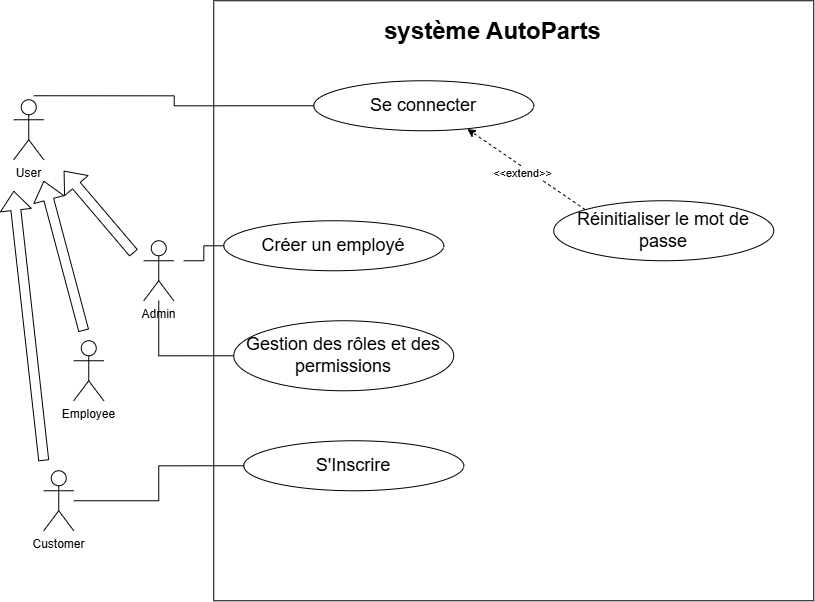
\includegraphics[width=0.8\textwidth]{images/uml/finaldiagramme.drawio.png}
    \caption{Diagramme de cas d'utilisation global du Sprint 1}
    \label{fig:usecase_sprint1}
\end{figure}

% ============================================================
% DESCRIPTION DES CAS D'UTILISATION
% ============================================================



\subsubsection{Description des Cas d’Utilisation}

Afin de compléter le diagramme de cas d’utilisation présenté précédemment, cette section décrit les principaux cas d’utilisation du sprint. Pour chaque cas, sont présentés les acteurs concernés, les préconditions, le scénario nominal, les postconditions ainsi que les principales exceptions.

%========================================================
% UC1
%========================================================

\subsubsection{UC1 : Se connecter}

Le cas d’utilisation « Se connecter » permet à un utilisateur d’accéder à son espace selon son profil et les autorisations qui lui sont attribuées. La description détaillée de ce cas d’utilisation est présentée dans le Tableau~\ref{tab:uc1}.

\begin{longtable}{|>{\raggedright\arraybackslash}p{4cm}|>{\raggedright\arraybackslash}p{10.5cm}|}

\caption{Description du cas d’utilisation « Se connecter »}
\label{tab:uc1}\\

\hline

\textbf{Élément} & \textbf{Description} \\

\hline

\textbf{Cas d’utilisation} & Se connecter \\

\hline

\textbf{Acteur(s)} & Utilisateur \\

\hline

\textbf{Préconditions} &
L'utilisateur possède un compte enregistré et dispose de ses identifiants de connexion. \\

\hline

\textbf{Scénario principal} &

1. L'utilisateur accède à l'interface de connexion. \newline
2. Il saisit son adresse e-mail et son mot de passe. \newline
3. Le système vérifie les informations d'authentification. \newline
4. Le système identifie le compte et vérifie son état. \newline
5. Le système authentifie l'utilisateur et génère un jeton JWT. \newline
6. Le système retourne les informations nécessaires à l'accès à l'application. \newline
7. L'utilisateur accède aux fonctionnalités autorisées selon son rôle et ses permissions. \\

\hline

\textbf{Postconditions} &
L'utilisateur est authentifié et dispose d'un jeton JWT permettant l'accès aux ressources protégées qui lui sont autorisées. \\

\hline

\textbf{Exceptions} &
Les identifiants sont incorrects, le compte est inactif ou une erreur d'authentification survient. \\

\hline

\end{longtable}

%========================================================
% UC2
%========================================================

\vspace{-0.2cm}

\subsubsection{UC2 : Réinitialiser le mot de passe}

Le cas d’utilisation « Réinitialiser le mot de passe » permet à un utilisateur ayant oublié son mot de passe de récupérer l’accès à son compte. Ce cas est déclenché depuis le cas « Se connecter » lorsque l’utilisateur sélectionne l’option de réinitialisation. La description détaillée de ce cas d’utilisation est présentée dans le Tableau~\ref{tab:uc2}.

\begin{longtable}{|>{\raggedright\arraybackslash}p{4cm}|>{\raggedright\arraybackslash}p{10.5cm}|}

\caption{Description du cas d’utilisation « Réinitialiser le mot de passe »}
\label{tab:uc2}\\

\hline

\textbf{Élément} & \textbf{Description} \\

\hline

\textbf{Cas d’utilisation} & Réinitialiser le mot de passe \\

\hline

\textbf{Acteur(s)} & Utilisateur \\

\hline

\textbf{Relation} &
Ce cas d’utilisation étend le cas « Se connecter » lorsque l’utilisateur sélectionne l’option « Mot de passe oublié ». \\

\hline

\textbf{Préconditions} &
L'utilisateur possède un compte enregistré dans le système et souhaite récupérer l'accès à son compte. \\

\hline

\textbf{Scénario principal} &

1. L'utilisateur accède à l'interface de connexion. \newline
2. Il sélectionne l'option « Mot de passe oublié ». \newline
3. Il saisit son adresse e-mail. \newline
4. Le système vérifie l'adresse e-mail et déclenche la procédure de réinitialisation. \newline
5. Le système génère un jeton de réinitialisation sécurisé. \newline
6. Le système envoie un e-mail contenant le lien de réinitialisation. \newline
7. L'utilisateur accède au lien reçu. \newline
8. Le système vérifie la validité du jeton. \newline
9. L'utilisateur saisit son nouveau mot de passe. \newline
10. Le système enregistre le nouveau mot de passe. \\

\hline

\textbf{Postconditions} &
Le mot de passe de l'utilisateur est réinitialisé et peut être utilisé lors d'une nouvelle authentification. \\

\hline

\textbf{Exceptions} &
L'adresse e-mail est invalide ou non associée à un compte, le jeton est invalide ou expiré, ou le nouveau mot de passe ne respecte pas les règles de sécurité. \\

\hline

\end{longtable}

%========================================================
% UC3
%========================================================

\vspace{-0.2cm}

\subsubsection{UC3 : S’inscrire}

Le cas d’utilisation « S’inscrire » permet à un client de créer son propre compte sur la plateforme. Après la création du compte, une vérification de l’adresse e-mail est effectuée afin de sécuriser son activation. La description détaillée de ce cas d’utilisation est présentée dans le Tableau~\ref{tab:uc3}.

\begin{longtable}{|>{\raggedright\arraybackslash}p{4cm}|>{\raggedright\arraybackslash}p{10.5cm}|}

\caption{Description du cas d’utilisation « S’inscrire »}
\label{tab:uc3}\\

\hline

\textbf{Élément} & \textbf{Description} \\

\hline

\textbf{Cas d’utilisation} & S’inscrire \\

\hline

\textbf{Acteur(s)} & Client \\

\hline

\textbf{Préconditions} &
Le client ne possède pas encore de compte et le formulaire d'inscription est accessible. \\

\hline

\textbf{Scénario principal} &

1. Le client accède au formulaire d'inscription. \newline
2. Il saisit les informations demandées. \newline
3. Le système vérifie la validité des données saisies. \newline
4. Le système vérifie que l'adresse e-mail n'est pas déjà utilisée. \newline
5. Le système crée le compte client. \newline
6. Le système génère un jeton de vérification. \newline
7. Le système envoie un e-mail contenant le lien de vérification. \newline
8. Le client accède au lien reçu afin de vérifier son adresse e-mail. \\

\hline

\textbf{Postconditions} &
Le compte client est créé et l'adresse e-mail est vérifiée après validation du lien reçu. Le client peut alors se connecter à son compte. \\

\hline

\textbf{Exceptions} &
L'adresse e-mail est déjà utilisée, les données saisies sont invalides ou le lien de vérification est invalide ou expiré. \\

\hline

\end{longtable}

%========================================================
% UC4
%========================================================

\vspace{-0.2cm}

\subsubsection{UC4 : Gérer les employés}

Le cas d’utilisation « Gérer les employés » regroupe les opérations permettant à l'administrateur de gérer les comptes des employés. Il inclut notamment la création d'un employé, la consultation de ses informations et la gestion de son compte. La description détaillée de ce cas d’utilisation est présentée dans le Tableau~\ref{tab:uc4}.

\begin{longtable}{|>{\raggedright\arraybackslash}p{4cm}|>{\raggedright\arraybackslash}p{10.5cm}|}

\caption{Description du cas d’utilisation « Gérer les employés »}
\label{tab:uc4}\\

\hline

\textbf{Élément} & \textbf{Description} \\

\hline

\textbf{Cas d’utilisation} & Gérer les employés \\

\hline

\textbf{Acteur(s)} & Administrateur \\

\hline

\textbf{Préconditions} &
L'administrateur est authentifié et dispose des droits nécessaires pour gérer les employés. \\

\hline

\textbf{Scénario principal} &

1. L'administrateur accède à l'interface de gestion des employés. \newline
2. Il sélectionne l'opération à effectuer. \newline
3. Lors de la création, il saisit les informations personnelles et professionnelles de l'employé. \newline
4. Le système vérifie la validité des données saisies. \newline
5. Le système crée le compte de l'employé. \newline
6. Le système attribue les informations professionnelles nécessaires, notamment le département et le rôle. \newline
7. Le système génère les informations de connexion initiales. \newline
8. Le système transmet les informations de connexion à l'employé par e-mail. \newline
9. L'administrateur peut ensuite consulter ou modifier les informations de l'employé selon les droits disponibles. \\

\hline

\textbf{Postconditions} &
Les informations de l'employé sont enregistrées dans le système et son compte est disponible. Lors d'une création, les informations de connexion sont transmises à l'employé. \\

\hline

\textbf{Exceptions} &
Les données saisies sont invalides, l'adresse e-mail est déjà utilisée ou l'administrateur ne dispose pas des autorisations nécessaires. \\

\hline

\end{longtable}

%========================================================
% UC5
%========================================================

\vspace{-0.2cm}

\subsubsection{UC5 : Gérer les rôles et les permissions}

Le cas d’utilisation « Gérer les rôles et les permissions » permet à l'administrateur de contrôler les autorisations accordées aux employés. Ces autorisations déterminent les fonctionnalités et les ressources auxquelles chaque utilisateur peut accéder. La description détaillée de ce cas d’utilisation est présentée dans le Tableau~\ref{tab:uc5}.

\begin{longtable}{|>{\raggedright\arraybackslash}p{4cm}|>{\raggedright\arraybackslash}p{10.5cm}|}

\caption{Description du cas d’utilisation « Gérer les rôles et les permissions »}
\label{tab:uc5}\\

\hline

\textbf{Élément} & \textbf{Description} \\

\hline

\textbf{Cas d’utilisation} & Gérer les rôles et les permissions \\

\hline

\textbf{Acteur(s)} & Administrateur \\

\hline

\textbf{Préconditions} &
L'administrateur est authentifié et dispose des droits d'administration nécessaires. \\

\hline

\textbf{Scénario principal} &

1. L'administrateur accède à l'interface de gestion des rôles et des permissions. \newline
2. Il sélectionne l'employé concerné. \newline
3. Il attribue ou modifie le rôle de l'employé. \newline
4. Il définit les permissions associées aux fonctionnalités autorisées. \newline
5. Le système vérifie les informations saisies. \newline
6. Le système enregistre les modifications. \newline
7. Les nouvelles autorisations sont prises en compte lors des accès aux ressources protégées. \\

\hline

\textbf{Postconditions} &
Le rôle et les permissions de l'employé sont mis à jour et les accès aux ressources sont contrôlés conformément aux nouvelles autorisations. \\

\hline

\textbf{Exceptions} &
L'administrateur ne dispose pas des droits nécessaires ou les informations saisies sont invalides. \\

\hline

\end{longtable}



\subsection{Diagrammes de Séquence}

Les diagrammes de séquence suivants illustrent le déroulement de deux fonctionnalités
principales liées à la gestion des employés : la création d'un employé par
l'administrateur et sa première authentification.


\subsubsection{Diagramme de Séquence : Création d'un Employé}

Le diagramme suivant décrit le processus de création d'un employé. L'administrateur saisit les informations nécessaires depuis l'interface Angular. La requête est ensuite transmise au backend Spring Boot, où les droits d'accès et les données sont vérifiés. Le système crée l'employé, son contrat ainsi que son solde de congés, puis envoie ses identifiants de connexion par e-mail.

La Figure~\ref{fig:sequence_employee} présente le diagramme de séquence correspondant à ce processus.

\begin{figure}[H]
    \centering
    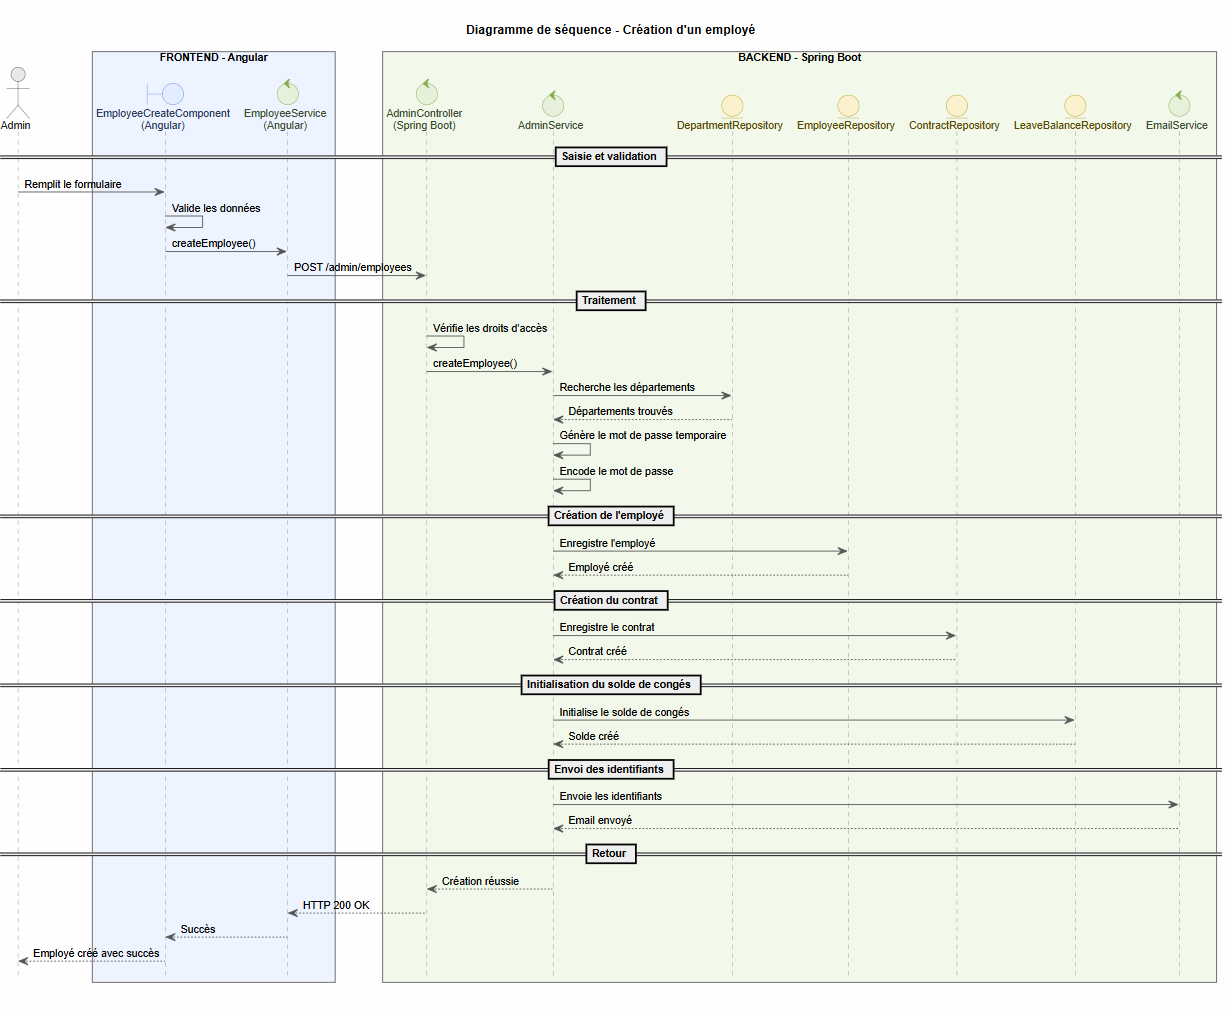
\includegraphics[
        angle=90,
        width=0.7\textheight
    ]{images/uml/seq1.png}
    \caption{Diagramme de séquence - Création d'un employé}
    \label{fig:sequence_employee}
\end{figure}



\subsubsection{Diagramme de Séquence : Première Authentification de l'Employé}

Le diagramme suivant présente le processus d'authentification d'un employé.

Après la saisie de ses identifiants, le système vérifie les informations d'authentification et génère un jeton JWT. Lors de la première connexion, l'employé est invité à modifier son mot de passe avant d'accéder au tableau de bord. En cas d'échec, le système retourne une erreur d'authentification. Ce processus est illustré par le diagramme de séquence présenté à la Figure~\ref{fig:sequence_first_authentication}.

\begin{figure}[H]
    \centering
    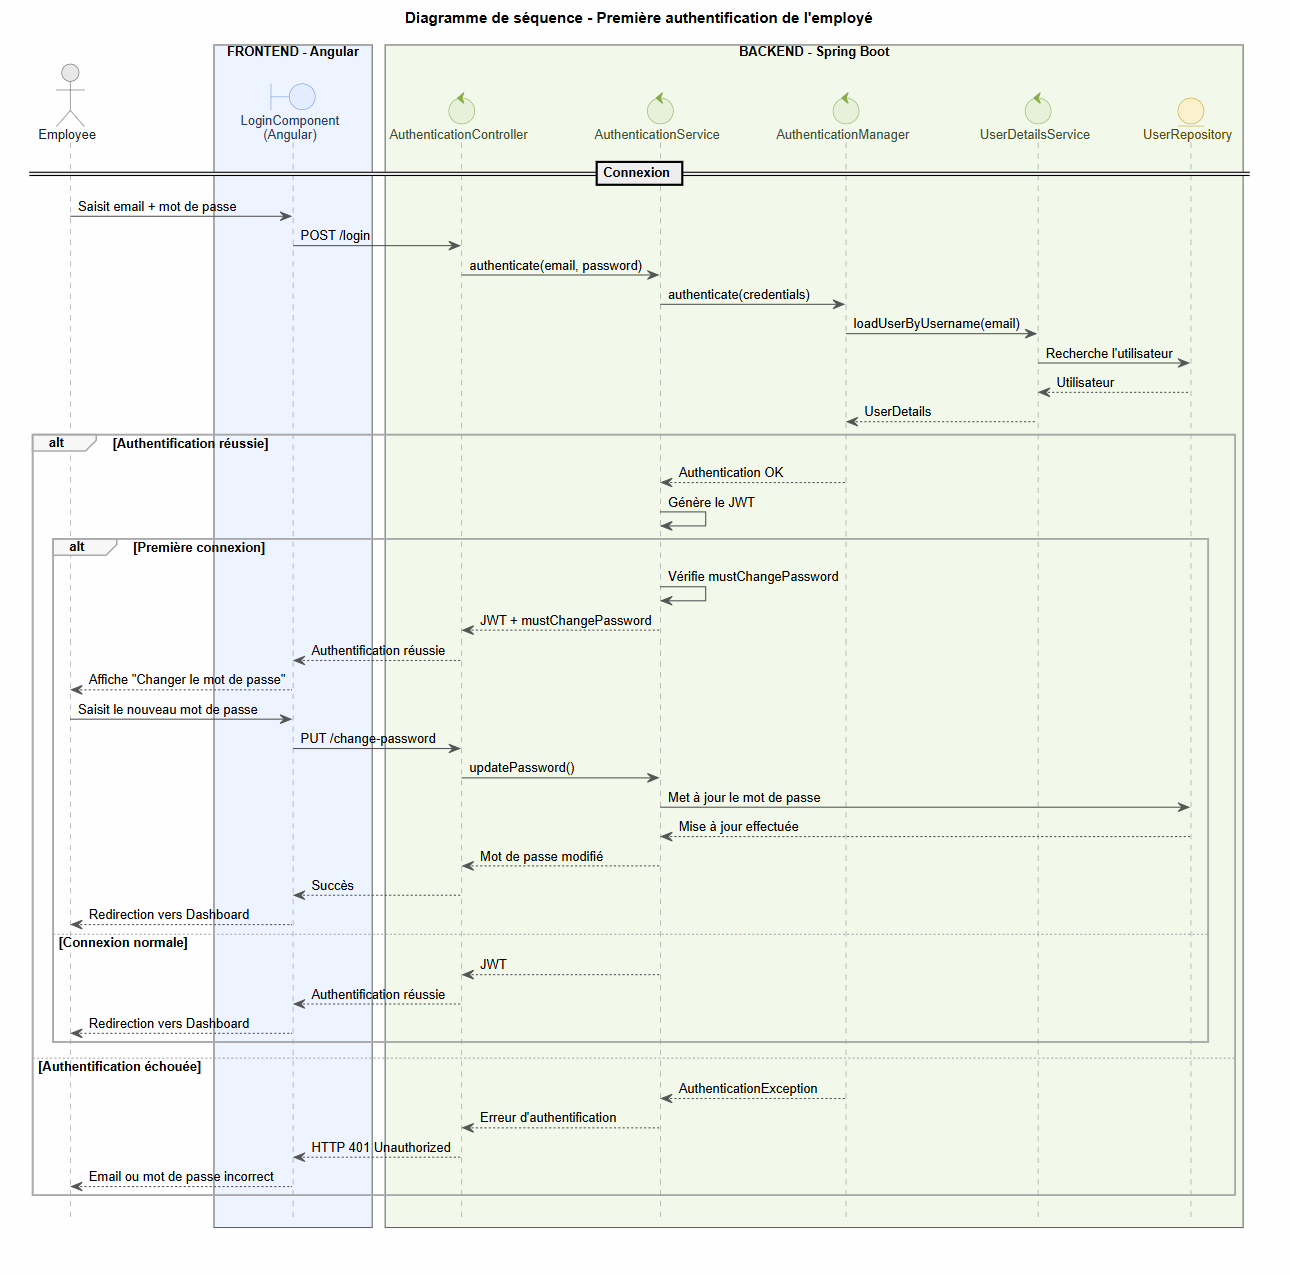
\includegraphics[width=1\textwidth]{images/uml/seq2.png}
    \caption{Diagramme de séquence - Première authentification de l'employé}
    \label{fig:sequence_first_authentication}
\end{figure}


\subsection{Diagramme de Classes} 
Le diagramme de classes présente la structure statique du module de gestion des utilisateurs. Il décrit les principales classes, leurs attributs ainsi que les relations qui existent entre elles. Les principales classes représentées sont : \begin{itemize} \item \textbf{User} : classe principale regroupant les informations communes à tous les utilisateurs, telles que l'identité, les informations de contact et les données liées à l'authentification. \item \textbf{Customer} : représente les clients de la plateforme et contient notamment leurs informations de fidélité. \item \textbf{Employee} : représente les employés du système et contient leurs informations professionnelles, leur disponibilité et leur statut. \item \textbf{Admin} : représente les administrateurs responsables de la gestion et de l'administration du système. \item \textbf{Department} : représente les différents départements auxquels les employés peuvent être affectés. \item \textbf{Permission} : représente les permissions disponibles dans le système et permet de définir les droits associés aux départements. \item \textbf{EmploymentStatus} : énumération permettant de représenter l'état d'un employé : \textit{ACTIVE}, \textit{ON\_LEAVE}, \textit{RESIGNED} ou \textit{TERMINATED}. \end{itemize} La structure et les relations entre ces différentes classes sont représentées dans le diagramme de classes présenté à la Figure~\ref{fig:class_diagram}.


\begin{figure}[H]
    \centering
    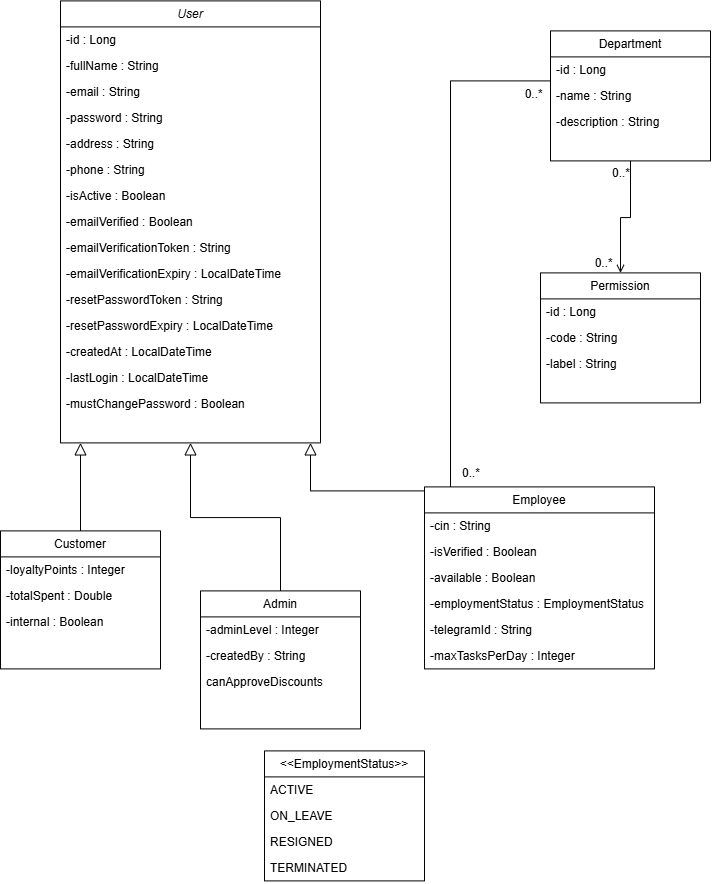
\includegraphics[width=0.6\textwidth]{images/uml/diagrammeClasseSprint1.drawio (1).png}
    \caption{Diagramme de classes - Gestion des utilisateurs}
    \label{fig:class_diagram}
\end{figure}









\section{Architecture de Sécurité}

La sécurité de l'application AutoParts repose sur l'intégration de \textit{Spring Security} et du mécanisme d'authentification basé sur le \ac{JWT} (\textit{JSON Web Token}). Cette architecture permet d'assurer l'authentification des utilisateurs, la protection des ressources exposées par les API REST ainsi que le contrôle des accès en fonction des rôles attribués à chaque utilisateur.

Comme illustré par la Figure~\ref{fig:architecture-jwt}, le processus de sécurité débute lors de la connexion de l'utilisateur. Après vérification des informations d'authentification, un jeton JWT est généré puis transmis au client. Ce jeton est ensuite utilisé pour accéder aux ressources protégées, où il est systématiquement vérifié avant l'autorisation de chaque requête.

\begin{figure}[H]
    \centering
    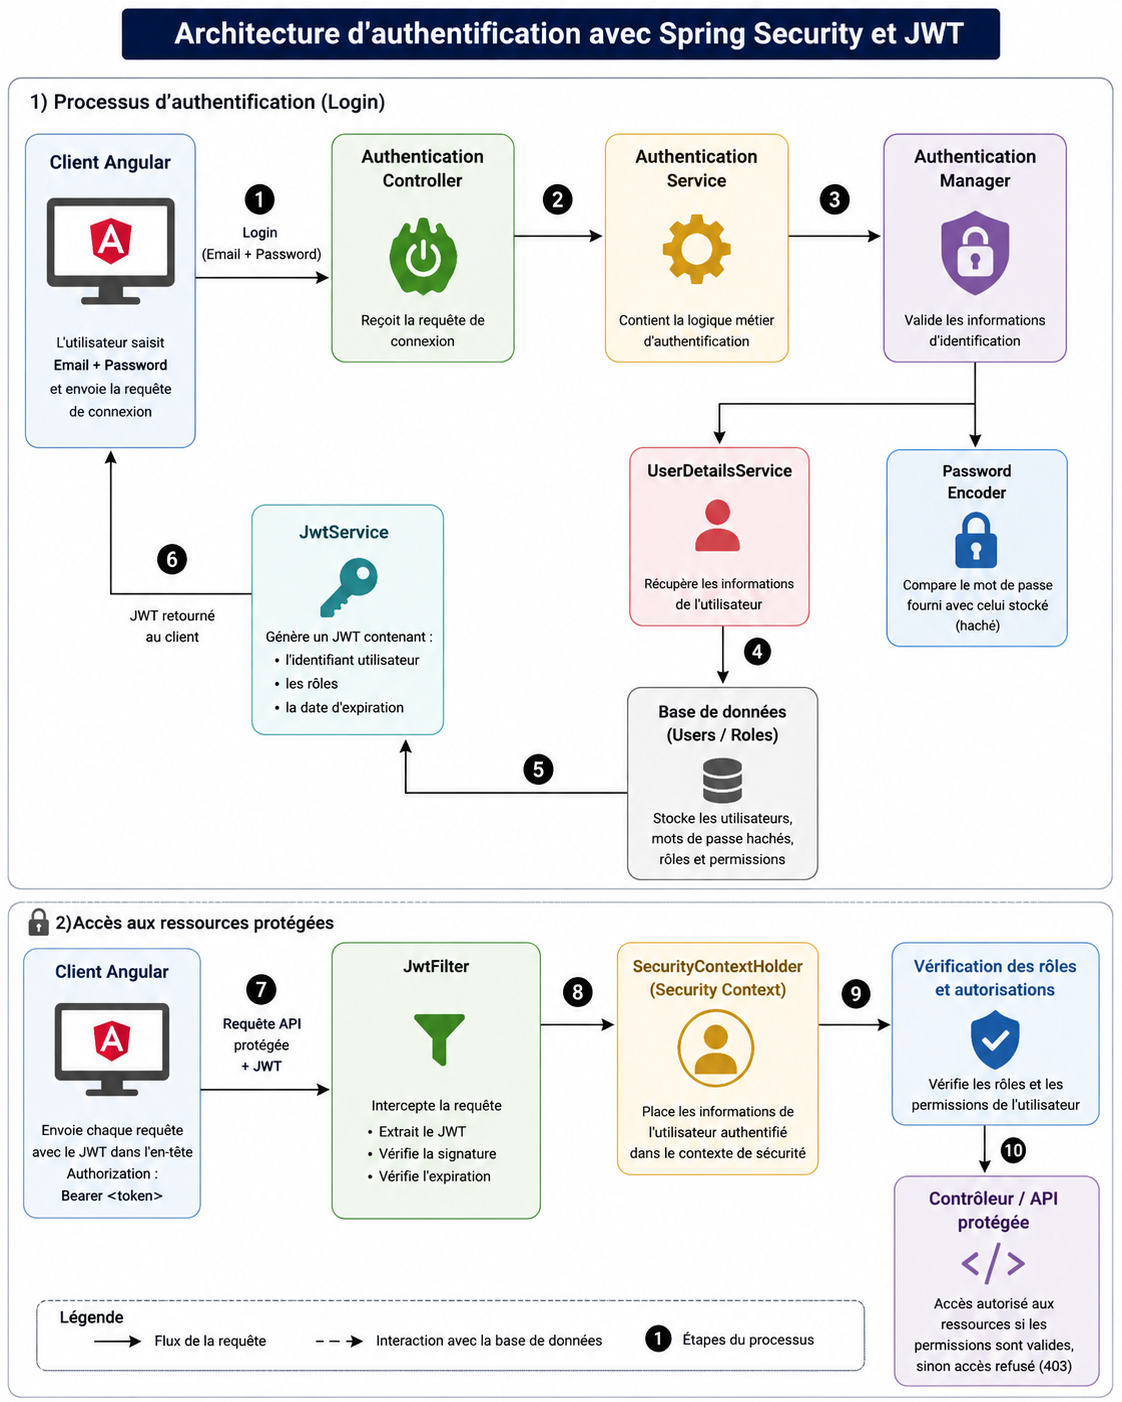
\includegraphics[width=0.8\textwidth]{images/architecture/archJWT.png}
    \caption{Architecture de sécurité basée sur Spring Security et JWT}
    \label{fig:architecture-jwt}
\end{figure}

\subsection{Architecture Spring Security}

Spring Security est un framework dédié à la sécurisation des applications Spring. Dans l'application MSG, il prend en charge l'authentification des utilisateurs, la protection des API et le contrôle des autorisations en fonction des rôles. Son fonctionnement repose principalement sur les composants suivants :

\begin{itemize}
    \item \textbf{Security Filter Chain} : intercepte chaque requête HTTP avant son traitement par l'application, vérifie la présence et la validité du JWT, identifie l'utilisateur authentifié et autorise ou refuse l'accès aux ressources protégées.
    \item \textbf{Authentication Provider} : valide les informations de connexion en recherchant l'utilisateur dans la base de données et en comparant le mot de passe fourni avec celui enregistré.
    \item \textbf{UserDetailsService} : récupère les informations nécessaires à l'authentification depuis la base de données, notamment l'identifiant, le mot de passe chiffré ainsi que les rôles associés.
    \item \textbf{PasswordEncoder} : assure le chiffrement des mots de passe avant leur stockage et permet une comparaison sécurisée lors de l'authentification.
\end{itemize}

Ces mécanismes s'appuient sur les recommandations de Spring Security \cite{springSecurityDoc,springInAction}.



\subsection{Authentification basée sur JWT}

Le \ac{JWT} (\textit{JSON Web Token}) est un standard permettant de transmettre de manière sécurisée les informations d'authentification entre le client et le serveur. Contrairement à une authentification basée sur les sessions, cette approche est \textit{stateless} : le serveur ne conserve pas l'état de connexion des utilisateurs, les informations nécessaires étant contenues dans le jeton.

Le processus d'authentification se déroule selon les étapes suivantes.

\begin{enumerate}
    \item L'utilisateur saisit son adresse e-mail et son mot de passe, qui sont envoyés au serveur.

    \item Les identifiants sont vérifiés à l'aide du \textit{UserDetailsService} et du \textit{PasswordEncoder}. Si les informations sont valides, l'utilisateur est authentifié.

    \item Le service \textit{JwtService} génère un jeton JWT contenant l'identifiant de l'utilisateur, son rôle ainsi que sa date d'expiration.

    \item Lors de chaque requête vers une ressource protégée, le client transmet ce jeton dans l'en-tête HTTP \texttt{Authorization}. Le filtre JWT valide alors le jeton avant de permettre l'accès à la ressource demandée.
\end{enumerate}

Cette approche améliore les performances des applications distribuées en supprimant la gestion des sessions côté serveur tout en garantissant un niveau élevé de sécurité des échanges \cite{jwtRFC}.


\section{Réalisation}

Cette section présente les principales fonctionnalités développées au cours de ce sprint concernant la gestion des utilisateurs et la sécurisation de l'application AutoParts. Elle décrit les différentes interfaces réalisées pour l'inscription des clients, l'authentification des utilisateurs, la réinitialisation des mots de passe ainsi que la création et la gestion des comptes des employés.

%%%%%%%%%%%%%%%%%%%%%%%%%%%%%%%%%%%%%%%%%%%%%%%%%%%%%%%%%%

\subsection{Inscription d'un Customer et vérification du compte par e-mail}

Le processus d'inscription permet à un \textbf{Customer} de créer un compte dans l'application en renseignant les informations demandées dans le formulaire d'inscription. Après validation des données, le système enregistre le nouvel utilisateur puis envoie automatiquement un e-mail de confirmation contenant un lien de vérification. Le compte n'est activé qu'après la validation de cette adresse électronique.

L'interface d'inscription développée permet au client de renseigner les informations nécessaires à la création de son compte, comme présenté dans la figure~\ref{fig:registerCustomer}.

\begin{figure}[H]
\centering
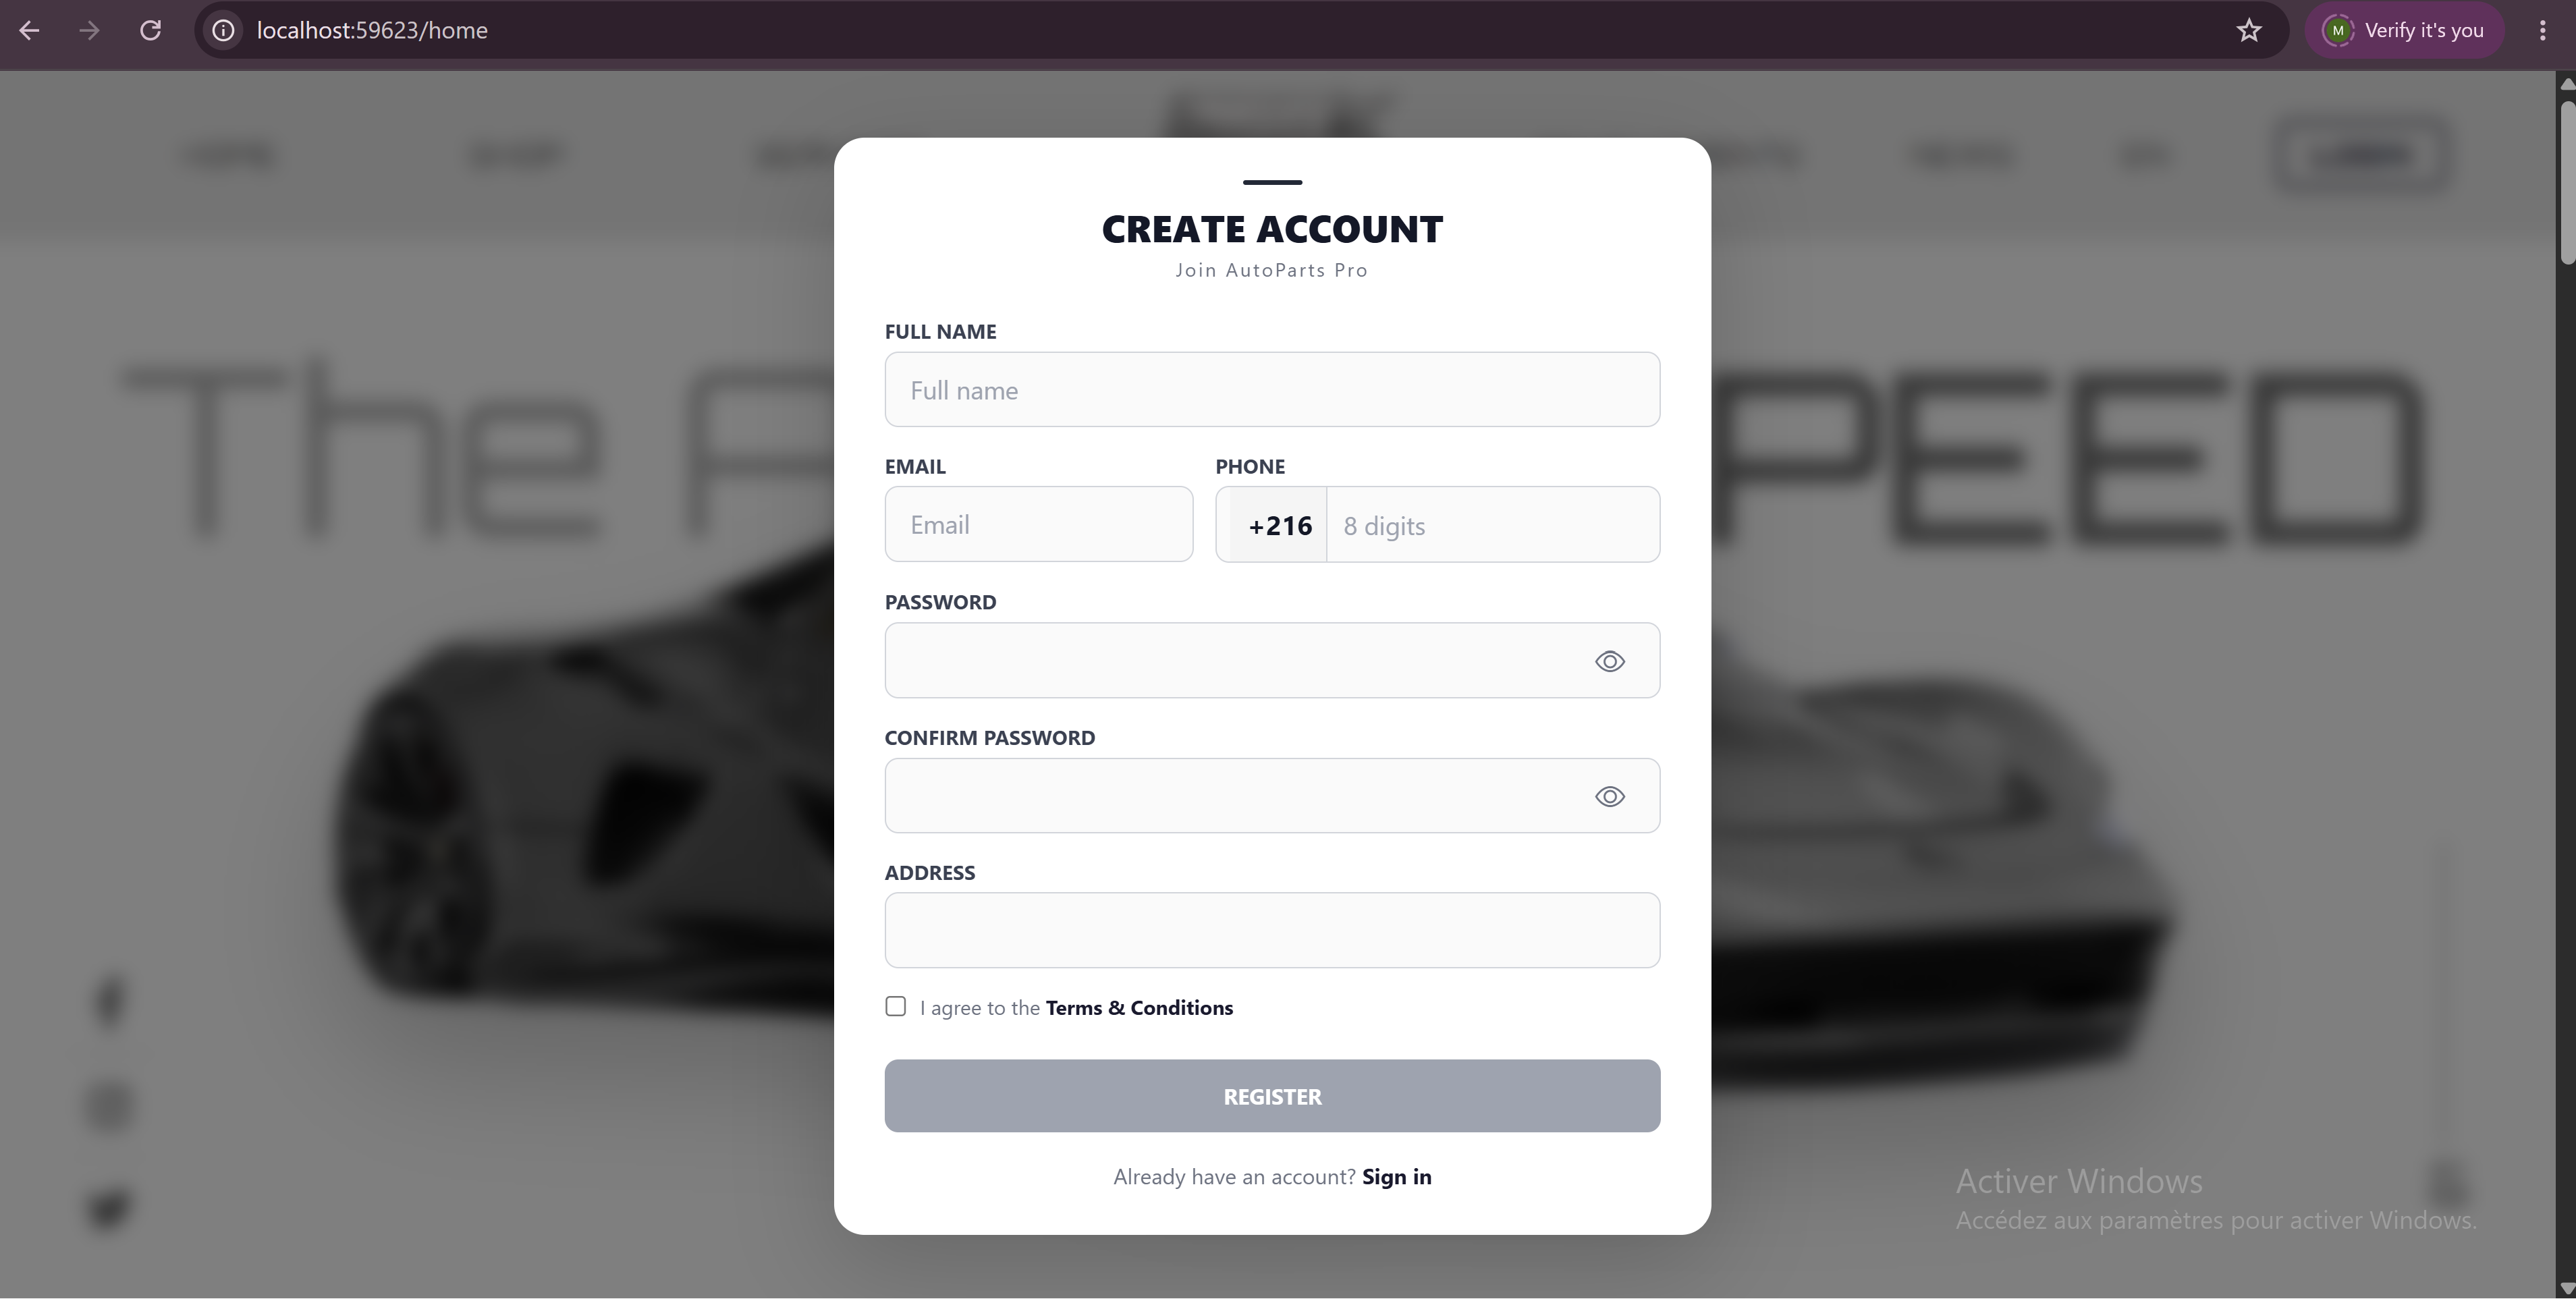
\includegraphics[width=0.75\textwidth]{images/interfaces/AuthCustomer/RegisterCustomer.png}
\caption{Interface d'inscription d'un Customer}
\label{fig:registerCustomer}
\end{figure}

Une fois le formulaire validé, le système crée le compte et déclenche l'envoi d'un e-mail de vérification. Le client doit alors utiliser le lien reçu afin de confirmer son adresse électronique avant de pouvoir accéder à son compte.

%---------------------------------------------------------

%%%%%%%%%%%%%%%%%%%%%%%%%%%%%%%%%%%%%%%%%%%%%%%%%%%%%%%%%%

\subsection{Authentification des utilisateurs}

L'interface de connexion permet aux différents utilisateurs de l'application (\textbf{Customer}, \textbf{Admin} et \textbf{Employee}) d'accéder à leurs espaces respectifs. Après la saisie des identifiants, Spring Security vérifie les informations de connexion puis génère un jeton JWT permettant d'accéder aux ressources protégées. Selon le rôle de l'utilisateur, celui-ci est automatiquement redirigé vers son interface dédiée.

Pour le côté e-commerce, l'interface d'authentification destinée au client est présentée dans la figure~\ref{fig:loginCustomer}. Elle permet au \textbf{Customer} de saisir son adresse e-mail et son mot de passe afin d'accéder à son espace personnel.

\begin{figure}[H]
\centering
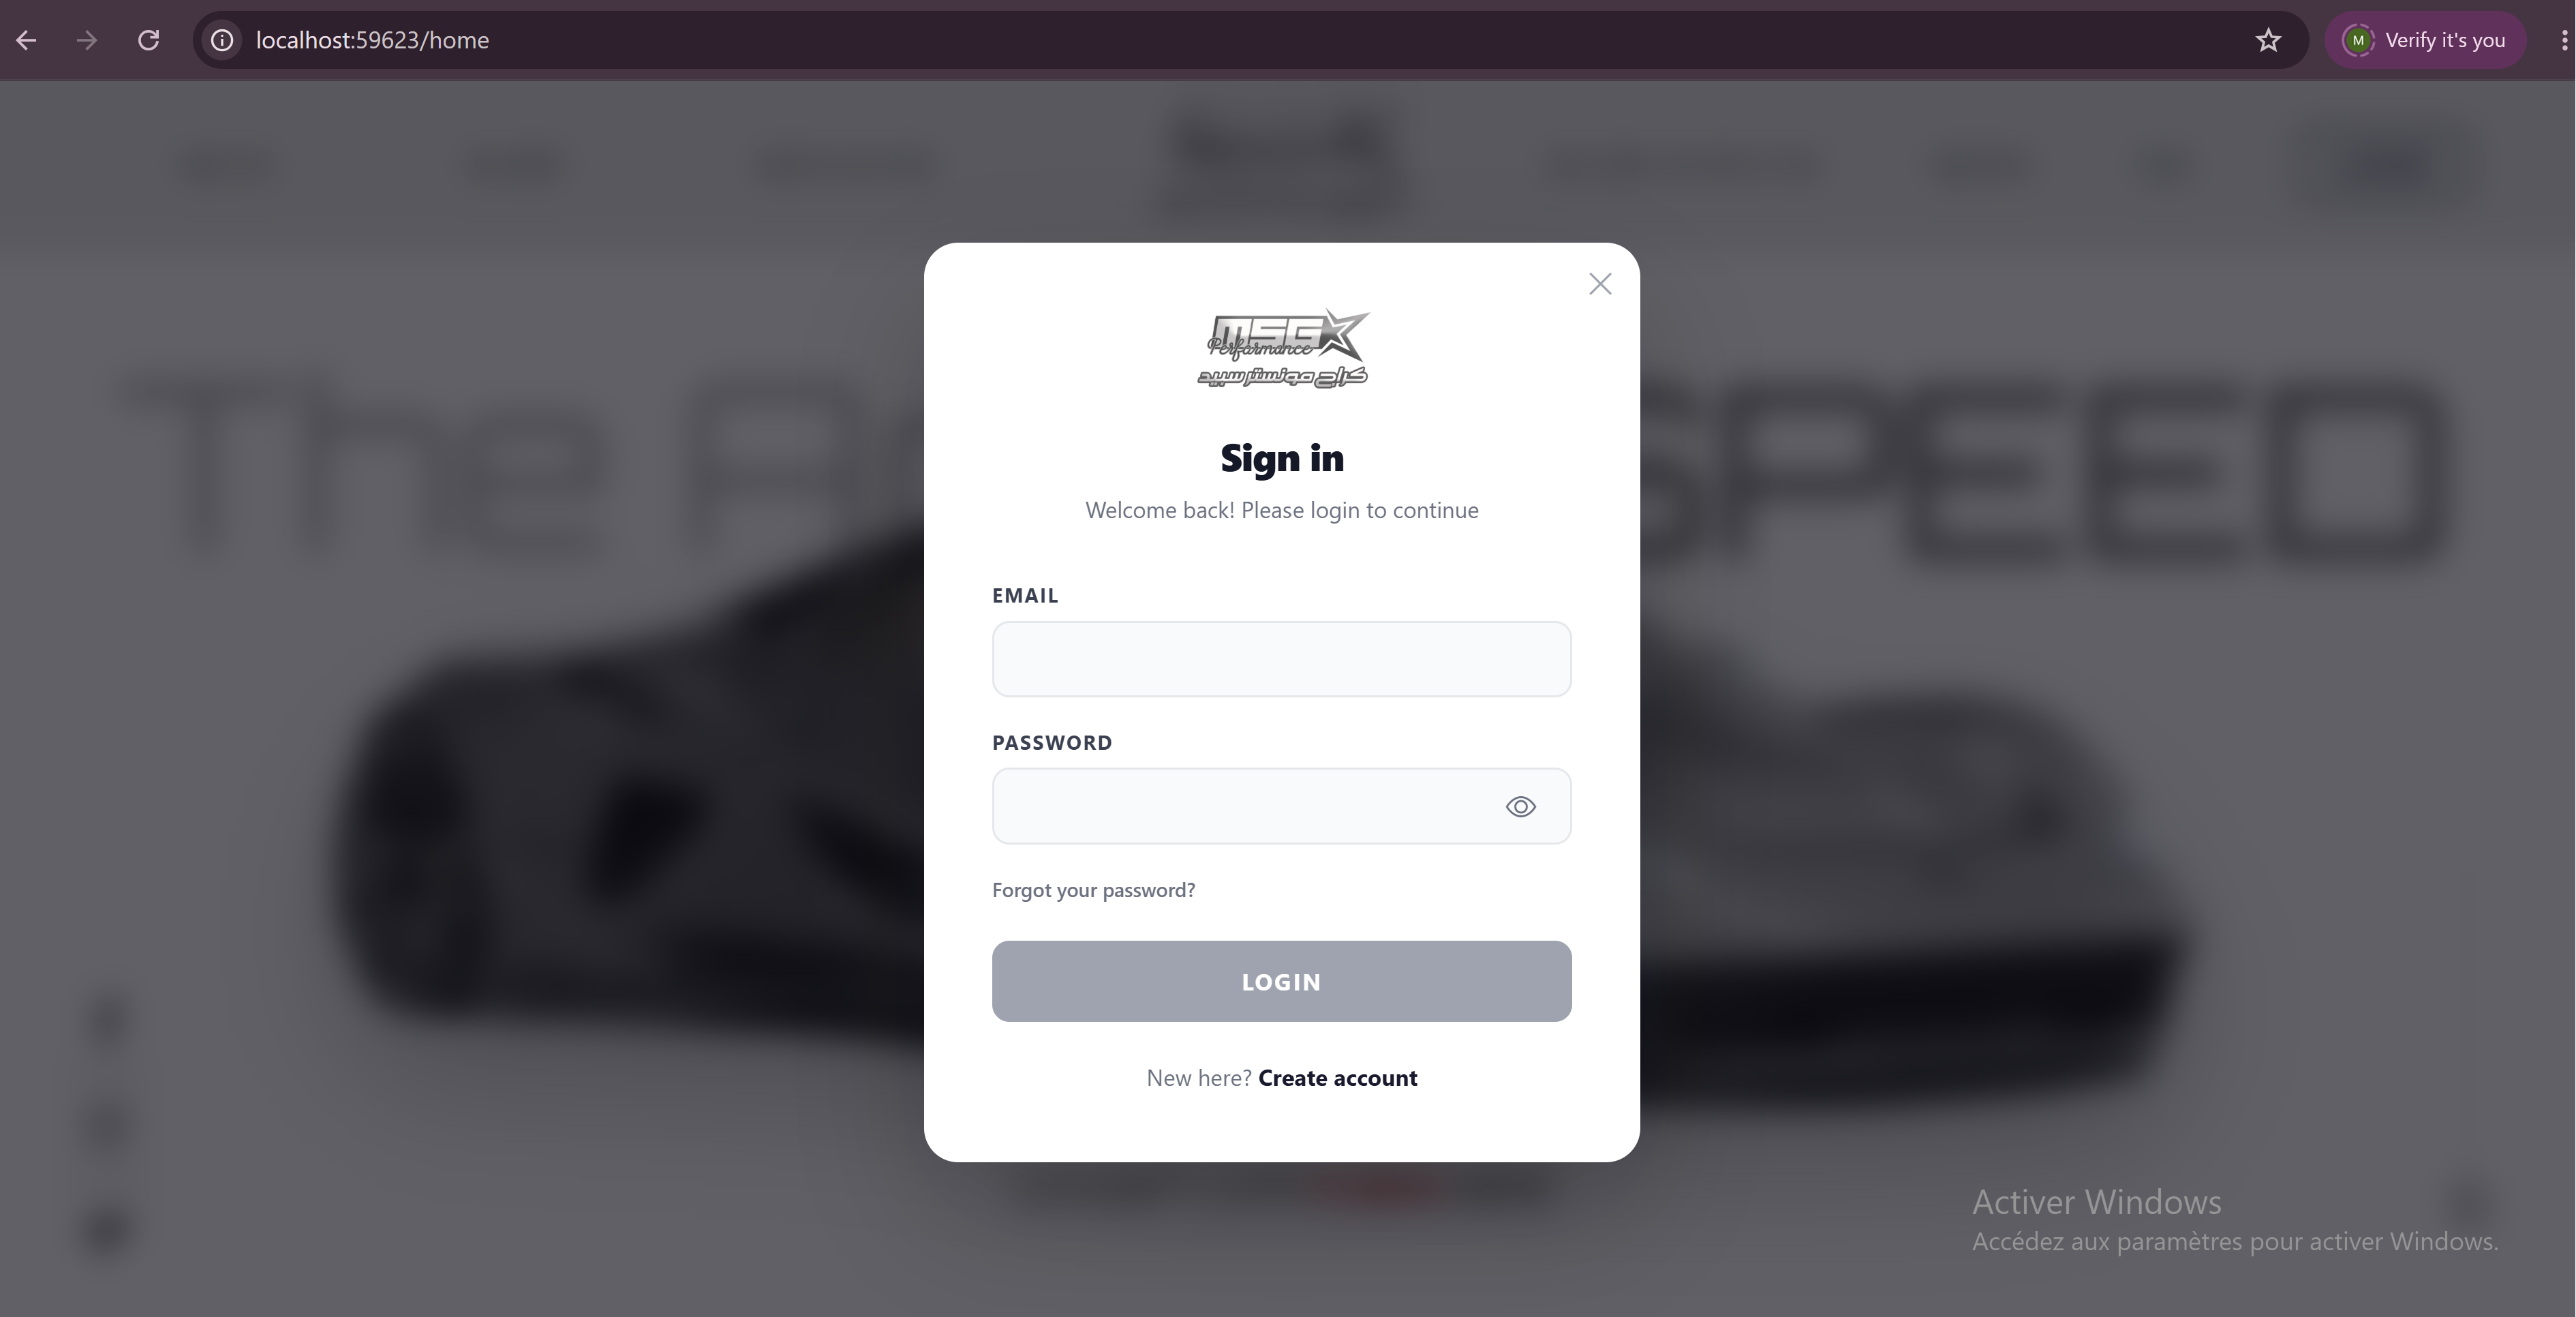
\includegraphics[width=0.75\textwidth]{images/interfaces/AuthCustomer/LOGINCUSTOMER.png}
\caption{Interface d'authentification du Client}
\label{fig:loginCustomer}
\end{figure}

Pour l'espace ERP, une interface de connexion commune permet à l'\textbf{Admin} et à l'\textbf{Employee} d'accéder à leurs espaces selon leurs rôles et leurs permissions. Cette interface est présentée dans la figure~\ref{fig:loginErp}.

\begin{figure}[H]
\centering
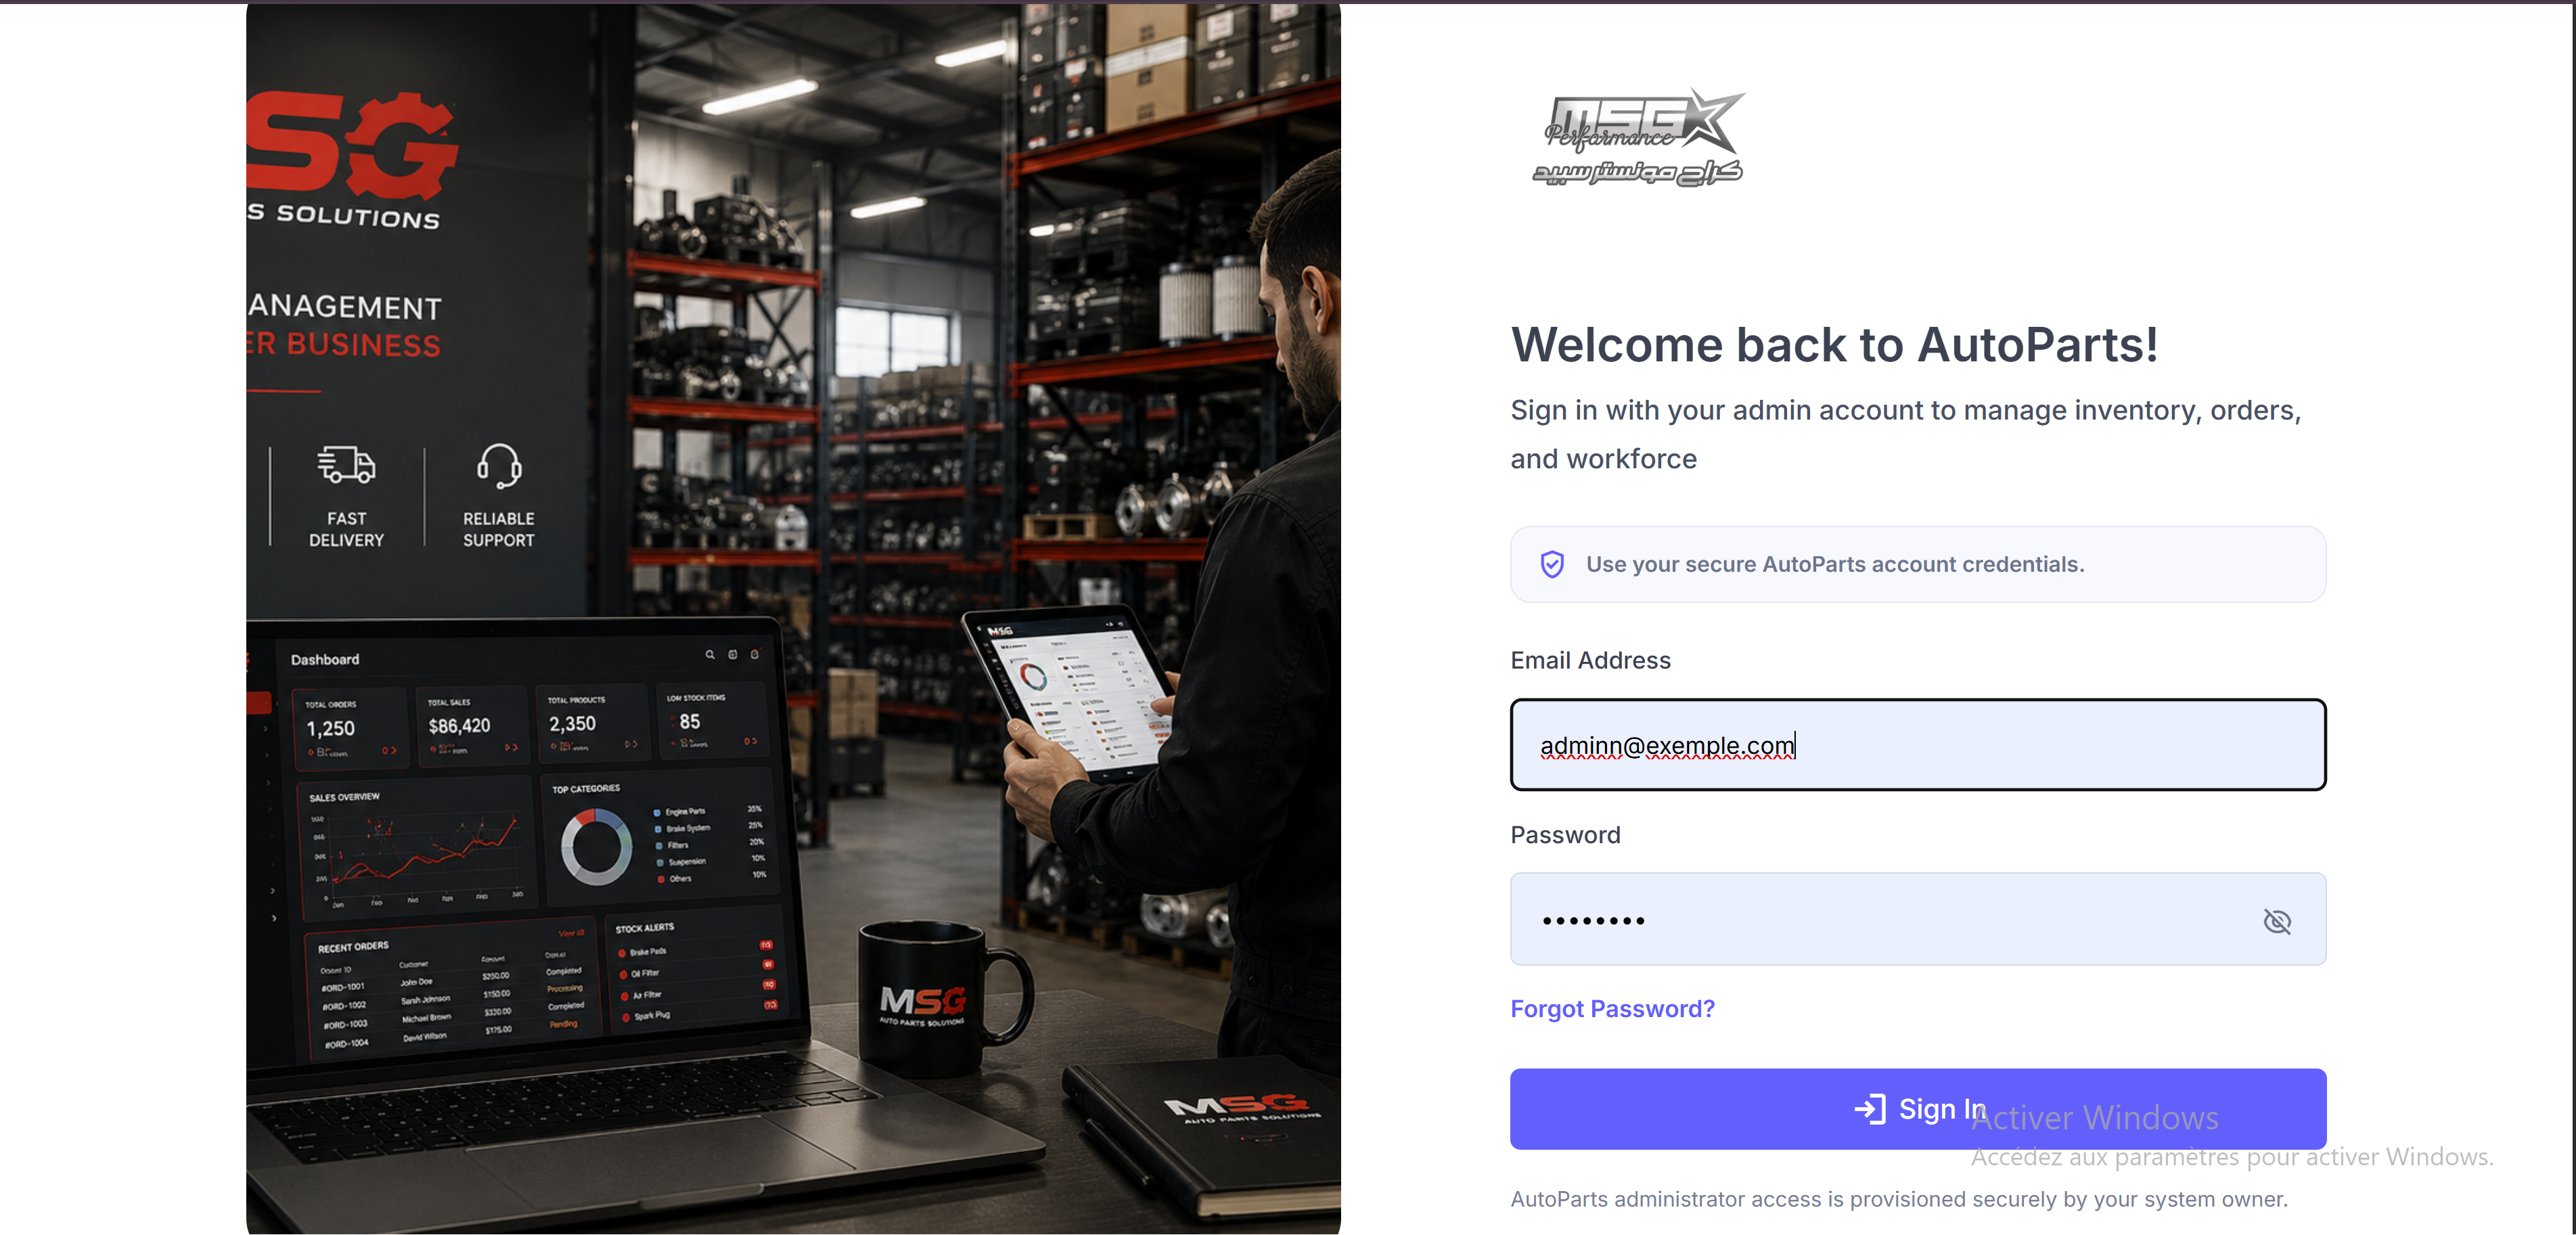
\includegraphics[width=0.75\textwidth]{images/interfaces/AuthErp/loginERP.png}
\caption{Interface d'authentification de l'Admin et de l'Employee}
\label{fig:loginErp}
\end{figure}

Après une authentification réussie, le système identifie le rôle de l'utilisateur et lui donne accès aux fonctionnalités qui lui sont autorisées.

%---------------------------------------------------------

%%%%%%%%%%%%%%%%%%%%%%%%%%%%%%%%%%%%%%%%%%%%%%%%%%%%%%%%%%

\subsection{Réinitialisation du mot de passe}

L'application offre une fonctionnalité permettant aux utilisateurs de récupérer l'accès à leur compte lorsqu'ils oublient leur mot de passe. Depuis l'interface de connexion, l'utilisateur sélectionne l'option de récupération du mot de passe et renseigne son adresse e-mail afin de recevoir un lien sécurisé de réinitialisation.

Du côté e-commerce, l'accès à cette fonctionnalité est proposé depuis l'interface de connexion du client, comme présenté dans la figure~\ref{fig:forgotPasswordCustomer}.

\begin{figure}[H]
\centering
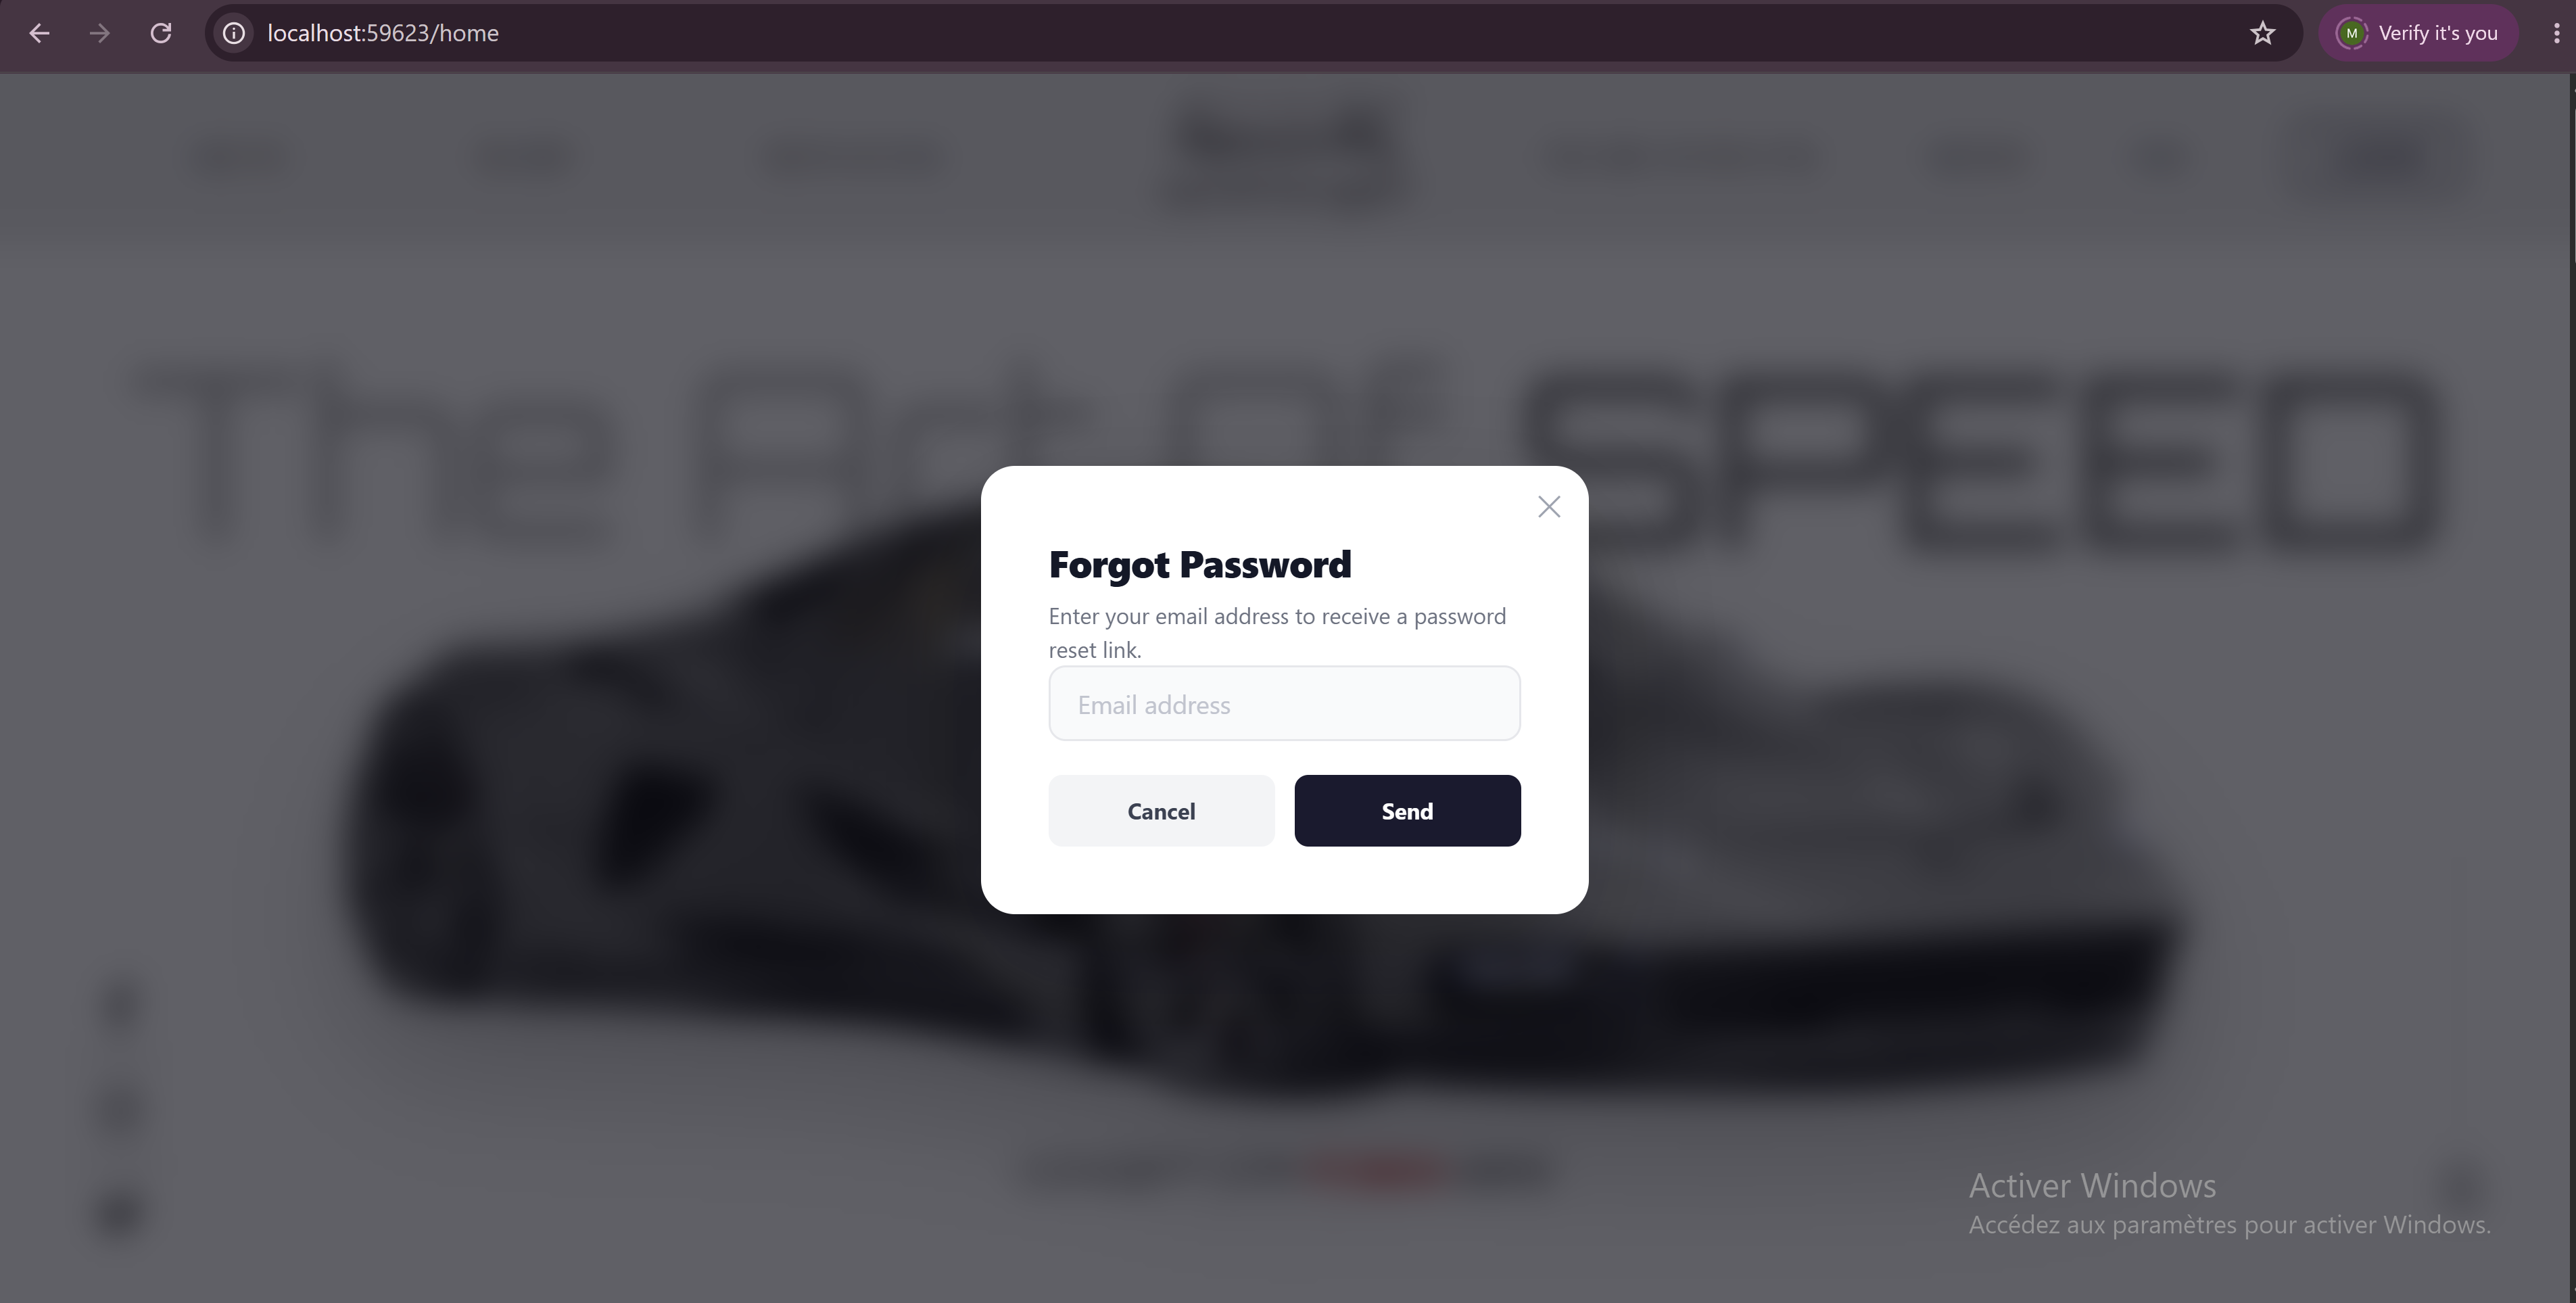
\includegraphics[width=0.75\textwidth]{images/interfaces/AuthCustomer/Forget_Password.png}
\caption{Interface de récupération du mot de passe du Client}
\label{fig:forgotPasswordCustomer}
\end{figure}

Une fonctionnalité équivalente est disponible dans l'espace ERP pour l'\textbf{Admin} et l'\textbf{Employee}. L'interface correspondante est illustrée dans la figure~\ref{fig:forgotPasswordErp}.

\begin{figure}[H]
\centering
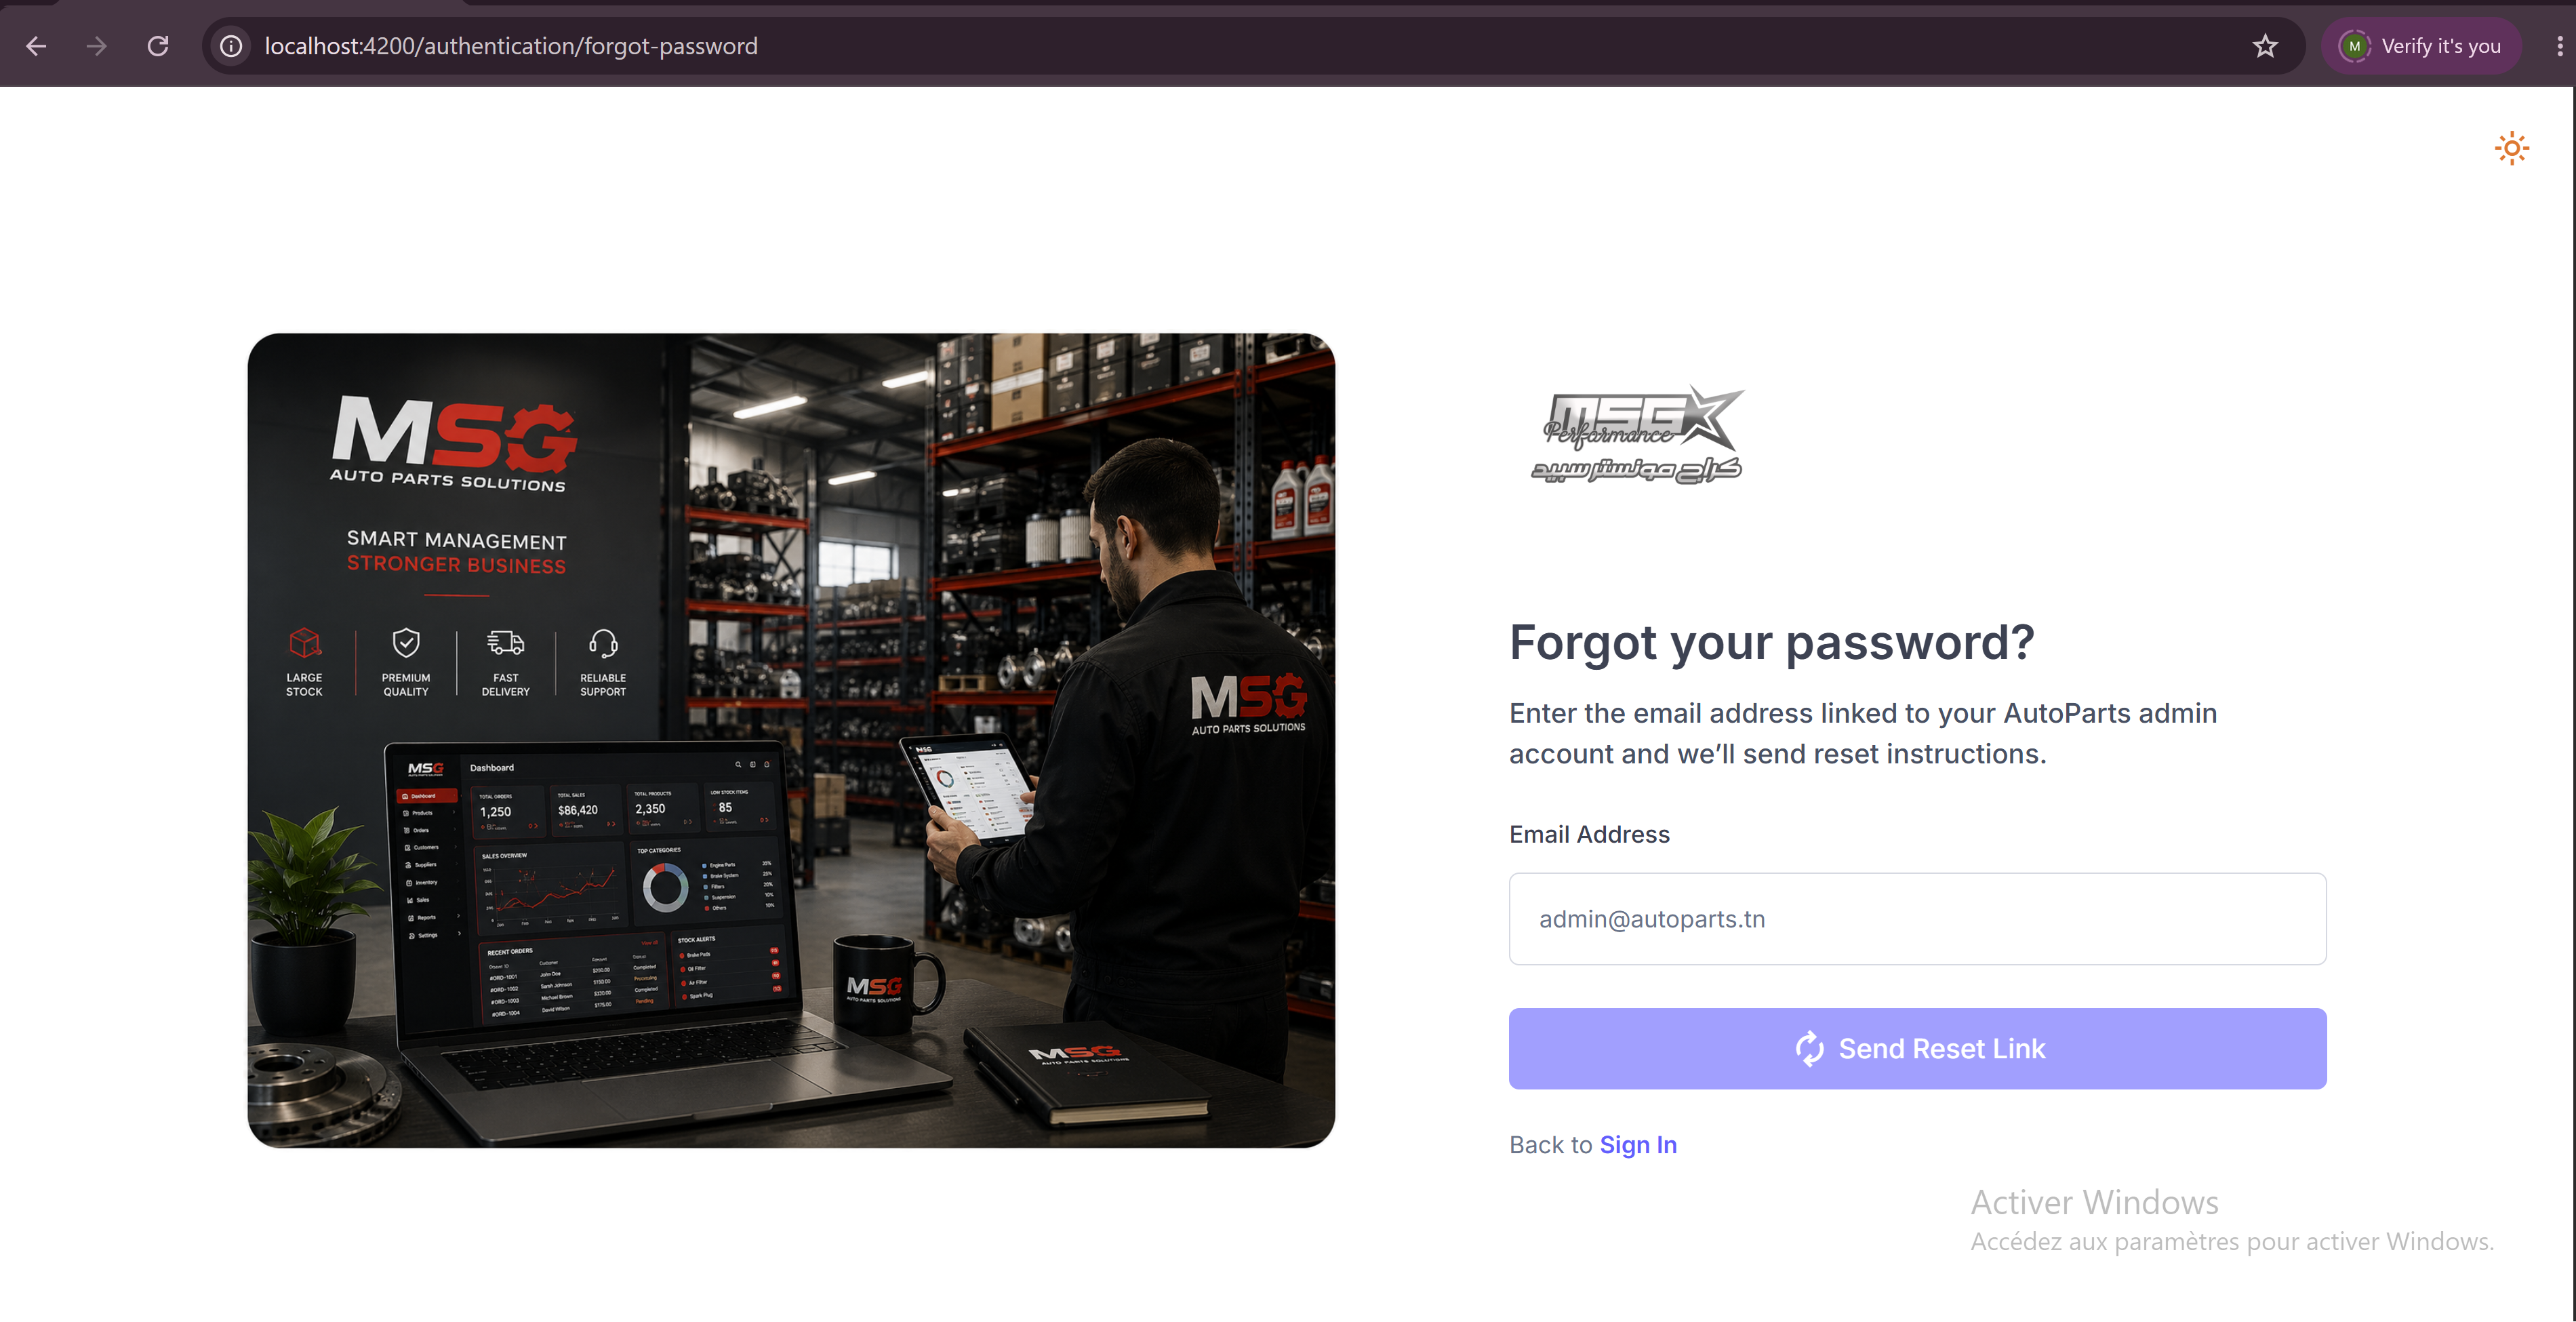
\includegraphics[width=0.75\textwidth]{images/interfaces/AuthErp/Forget_PasswordERP.png}
\caption{Interface de récupération du mot de passe de l'Admin et de l'Employee}
\label{fig:forgotPasswordErp}
\end{figure}

Après la demande de réinitialisation, le système génère un lien sécurisé envoyé à l'adresse e-mail associée au compte. L'utilisateur accède ensuite à ce lien afin de définir un nouveau mot de passe.

L'interface permettant de saisir le nouveau mot de passe pour un client est présentée dans la figure~\ref{fig:resetPasswordClient}.

\begin{figure}[H]
\centering
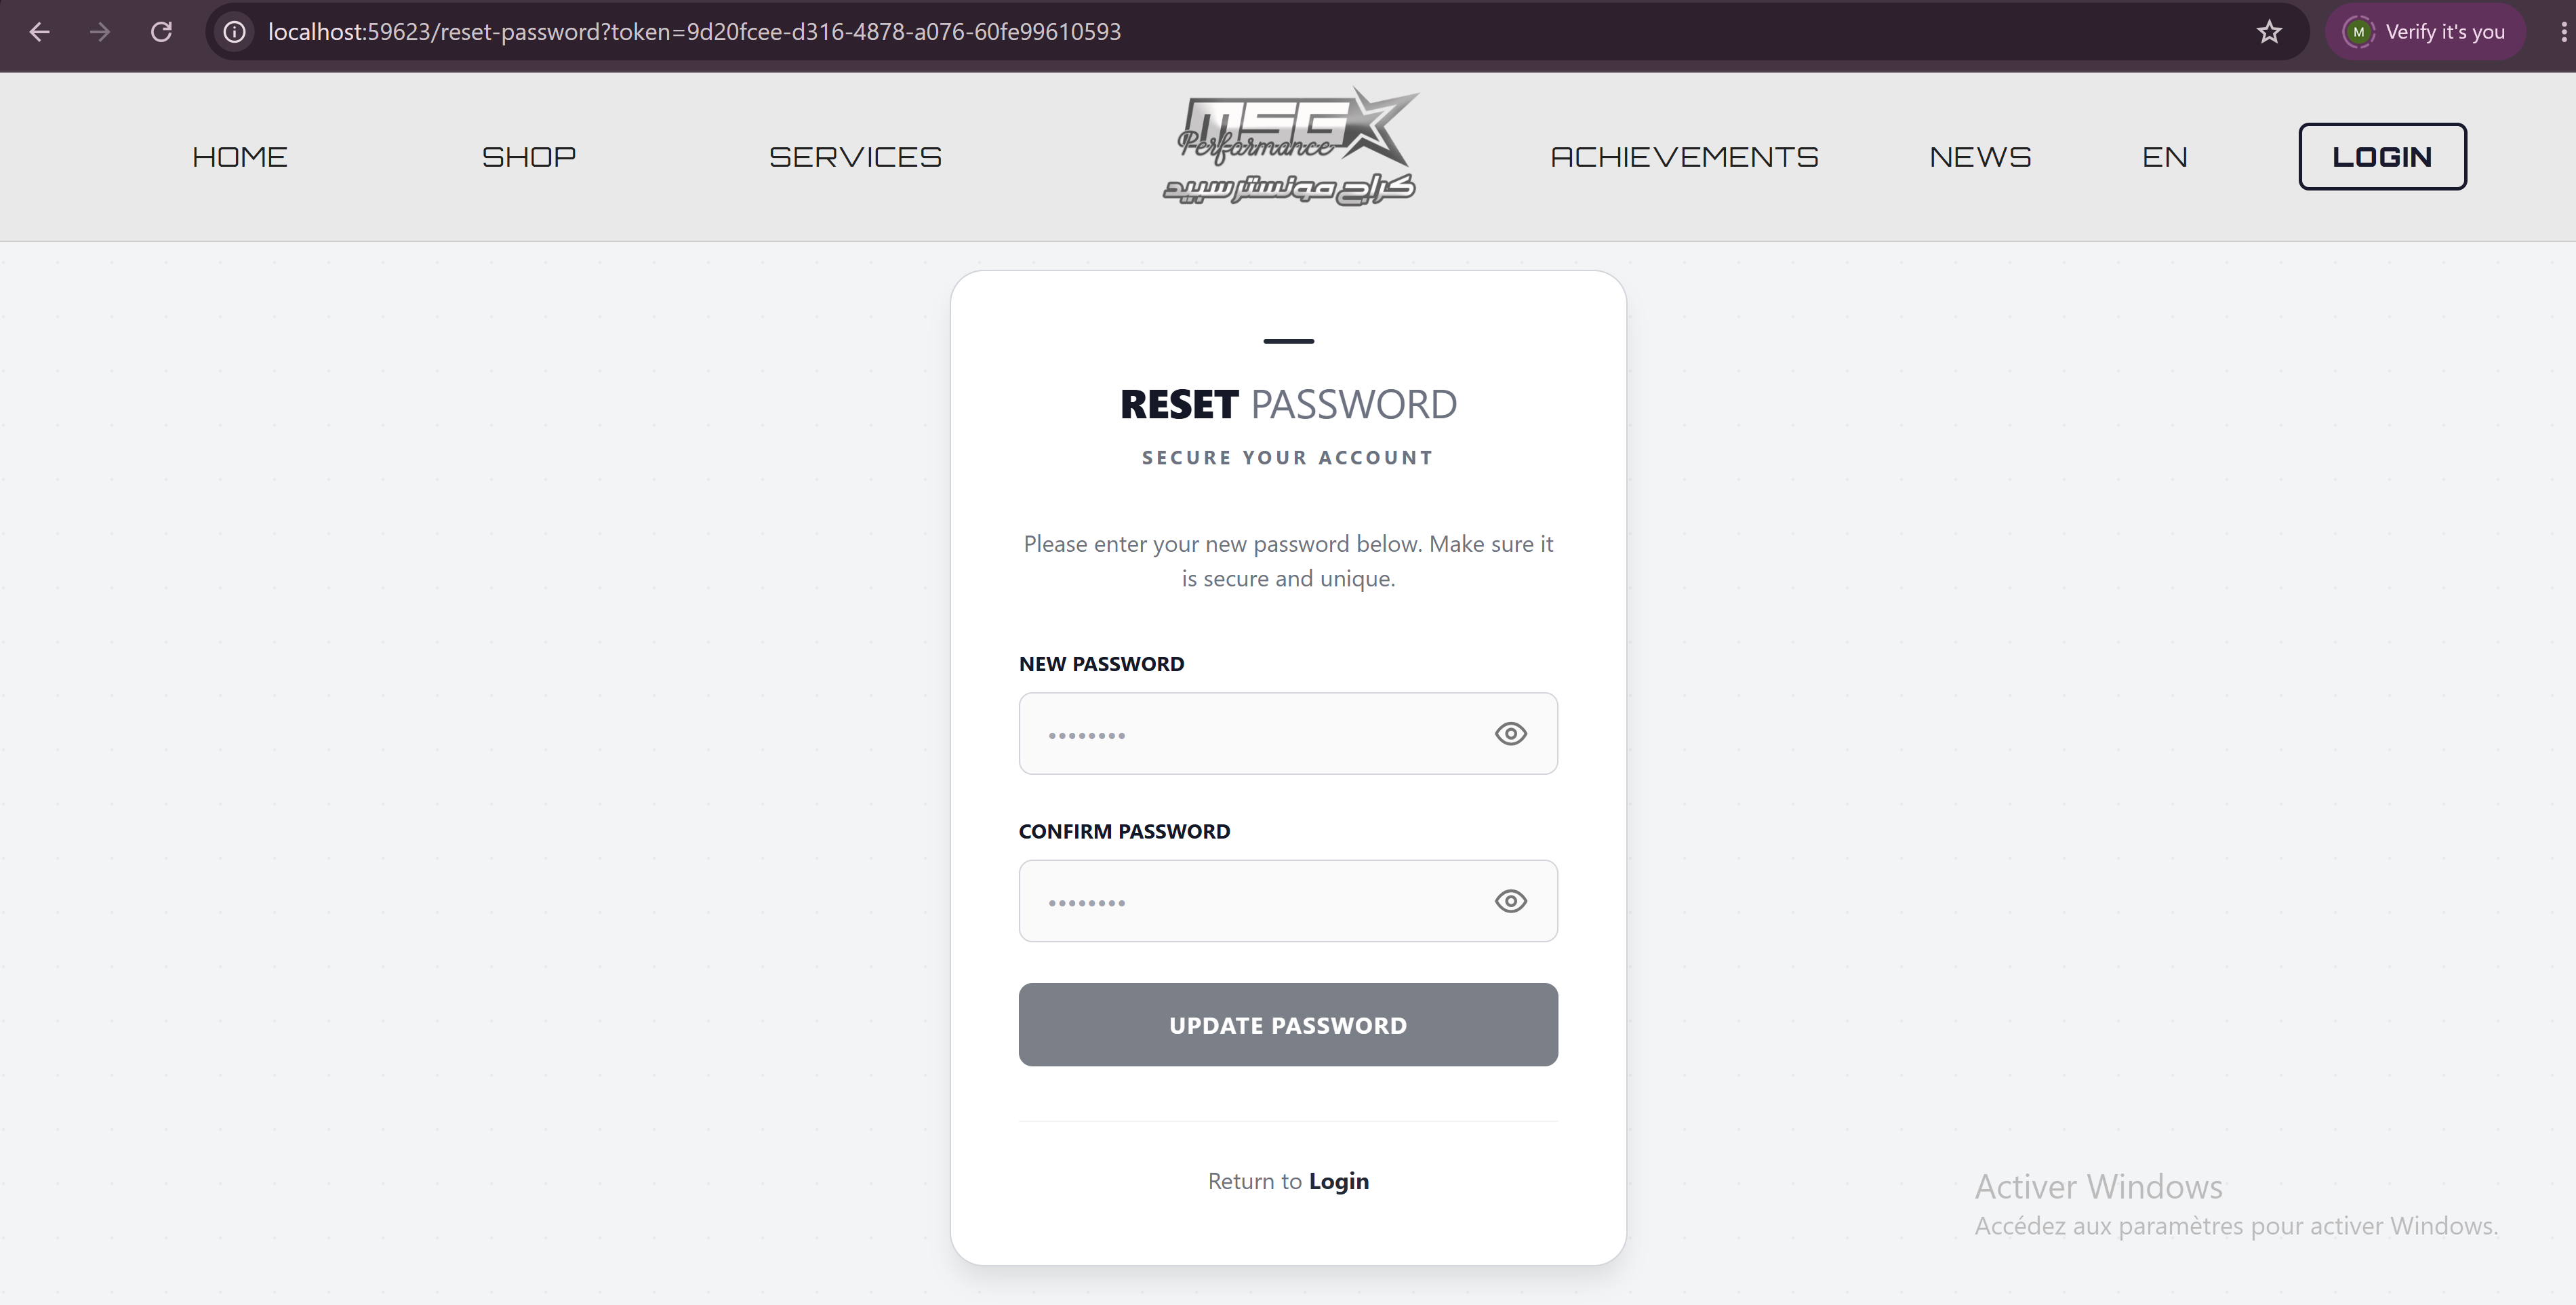
\includegraphics[width=0.75\textwidth]{images/interfaces/AuthCustomer/Reset_Password.png}
\caption{Interface de réinitialisation du mot de passe du Client}
\label{fig:resetPasswordClient}
\end{figure}

Pour les utilisateurs de l'espace ERP, l'interface de définition du nouveau mot de passe est présentée dans la figure~\ref{fig:resetPasswordErp}.

\begin{figure}[H]
\centering
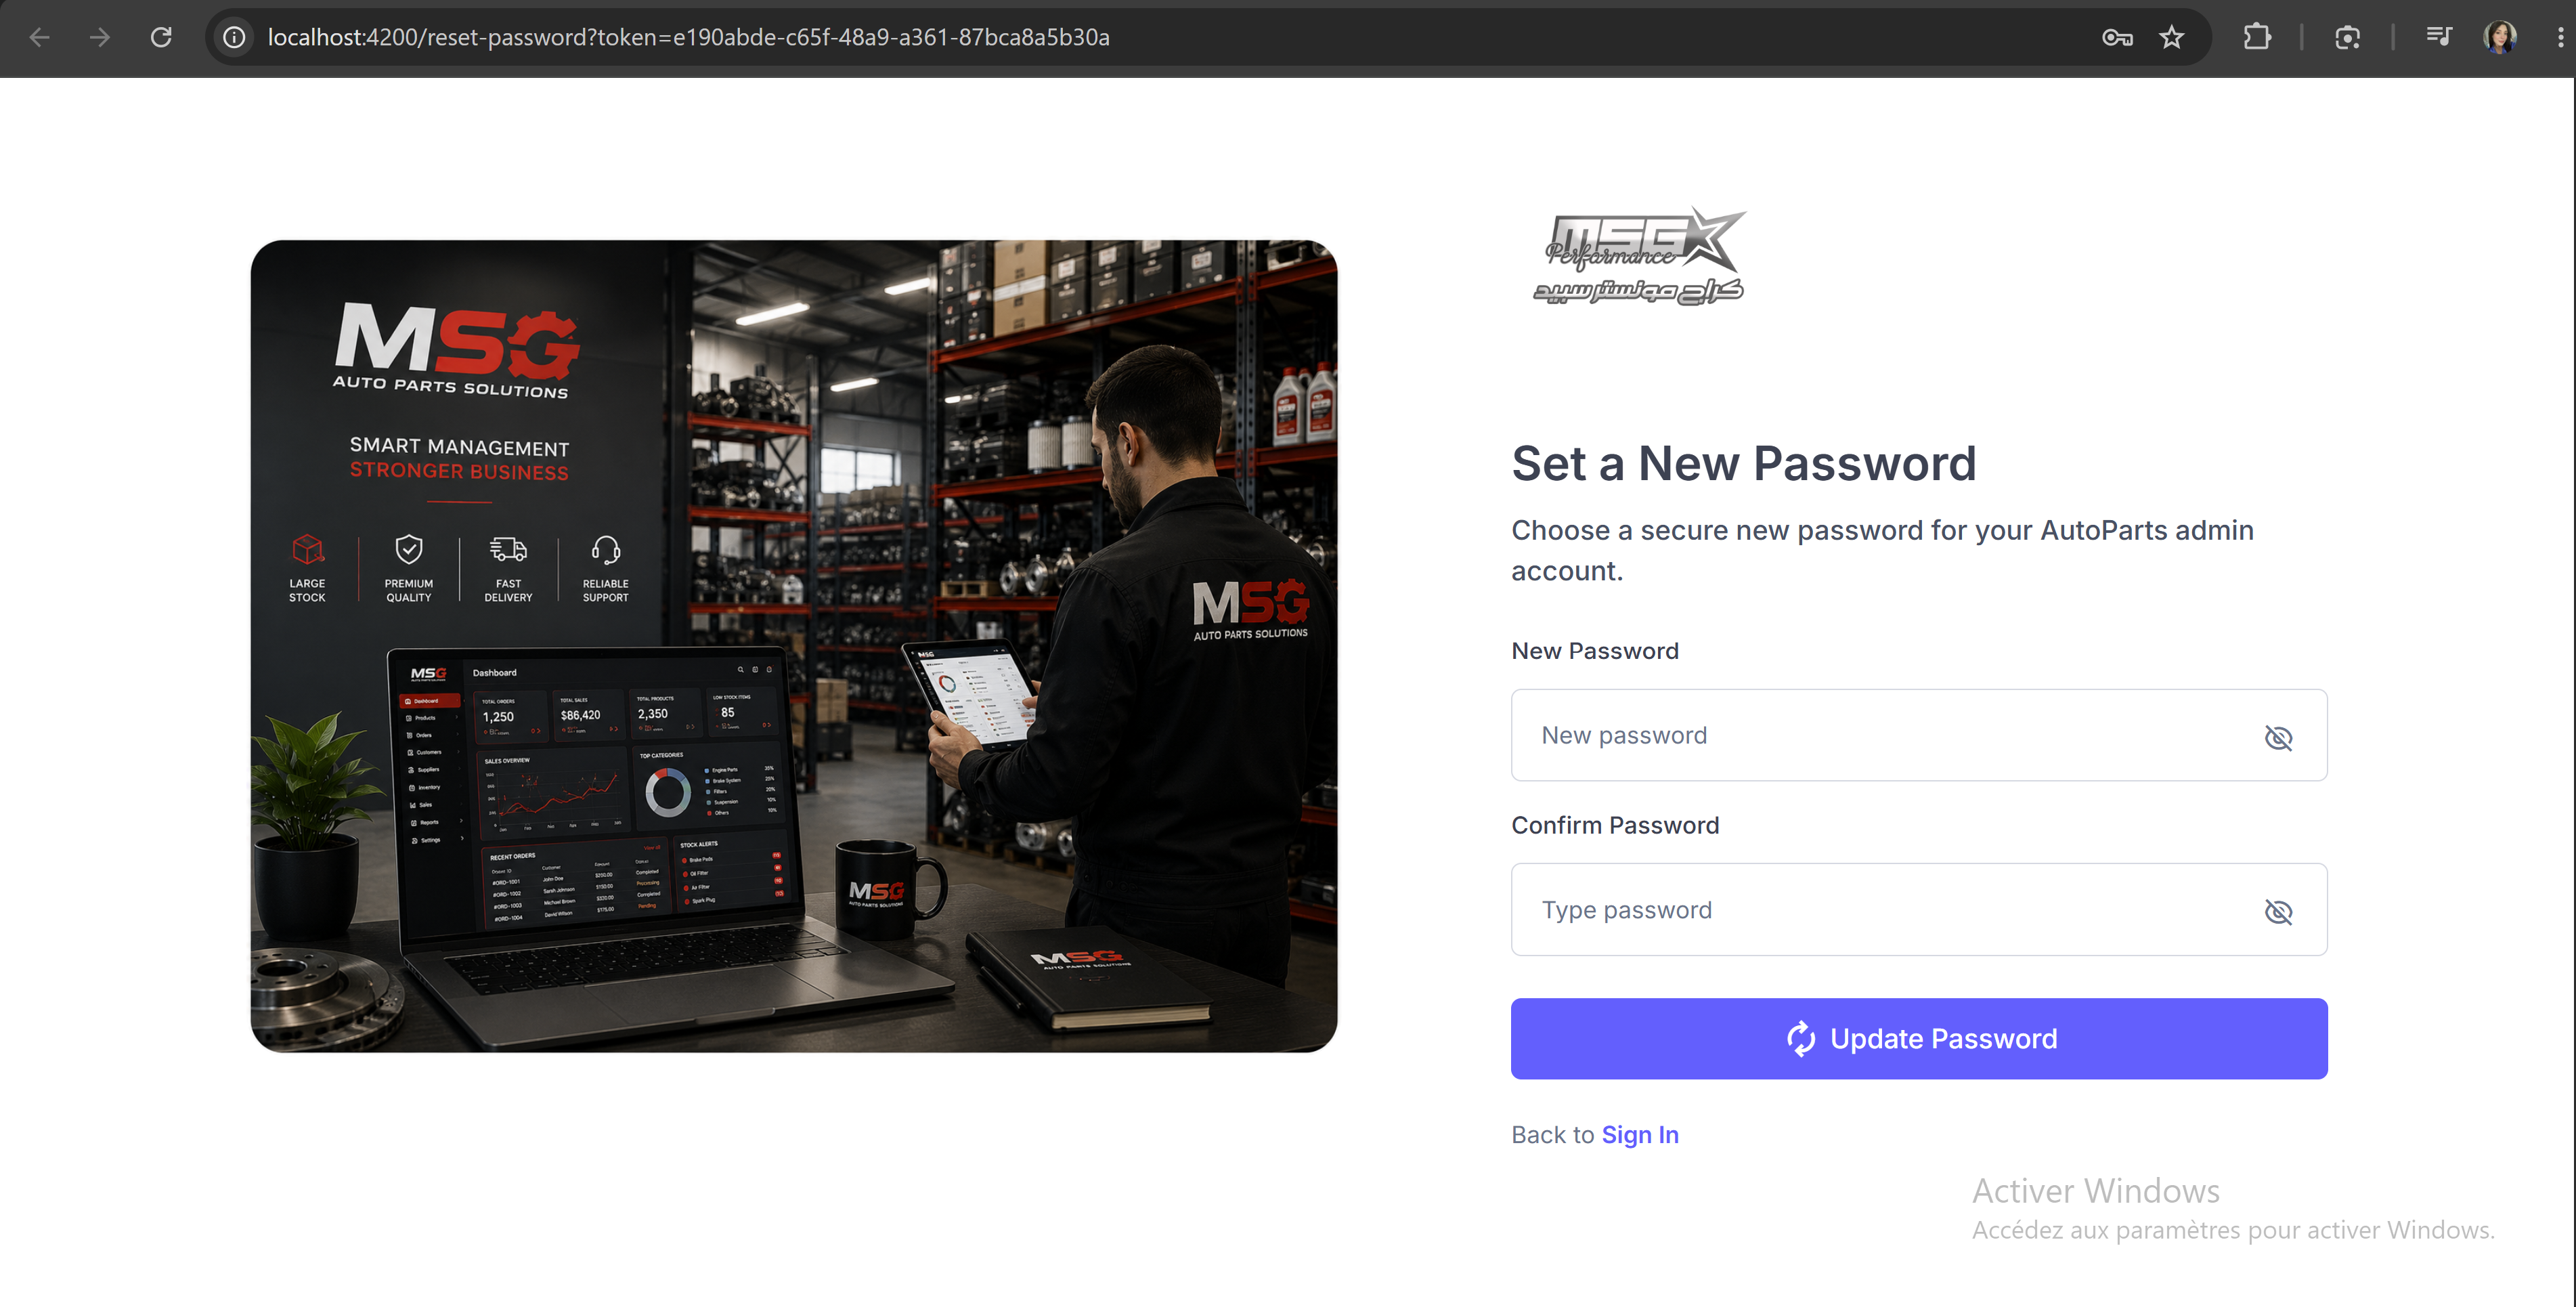
\includegraphics[width=0.75\textwidth]{images/interfaces/AuthErp/Reset_PasswordERP.png}
\caption{Interface de réinitialisation du mot de passe de l'Admin et de l'Employee}
\label{fig:resetPasswordErp}
\end{figure}

Le système vérifie la validité du jeton de réinitialisation avant d'autoriser la modification du mot de passe. Une fois l'opération terminée, l'utilisateur peut de nouveau s'authentifier avec ses nouvelles informations d'accès.

%---------------------------------------------------------

%%%%%%%%%%%%%%%%%%%%%%%%%%%%%%%%%%%%%%%%%%%%%%%%%%%%%%%%%%

\subsection{Création et initialisation d'un Employee}

Contrairement au \textbf{Customer}, un \textbf{Employee} ne crée pas son compte lui-même. Celui-ci est créé par l'\textbf{Admin} à partir de l'interface de gestion des employés.

L'interface de création permet à l'administrateur de renseigner les informations nécessaires concernant le nouvel employé. Cette interface est présentée dans la figure~\ref{fig:createEmployee}.

\begin{figure}[H]
\centering
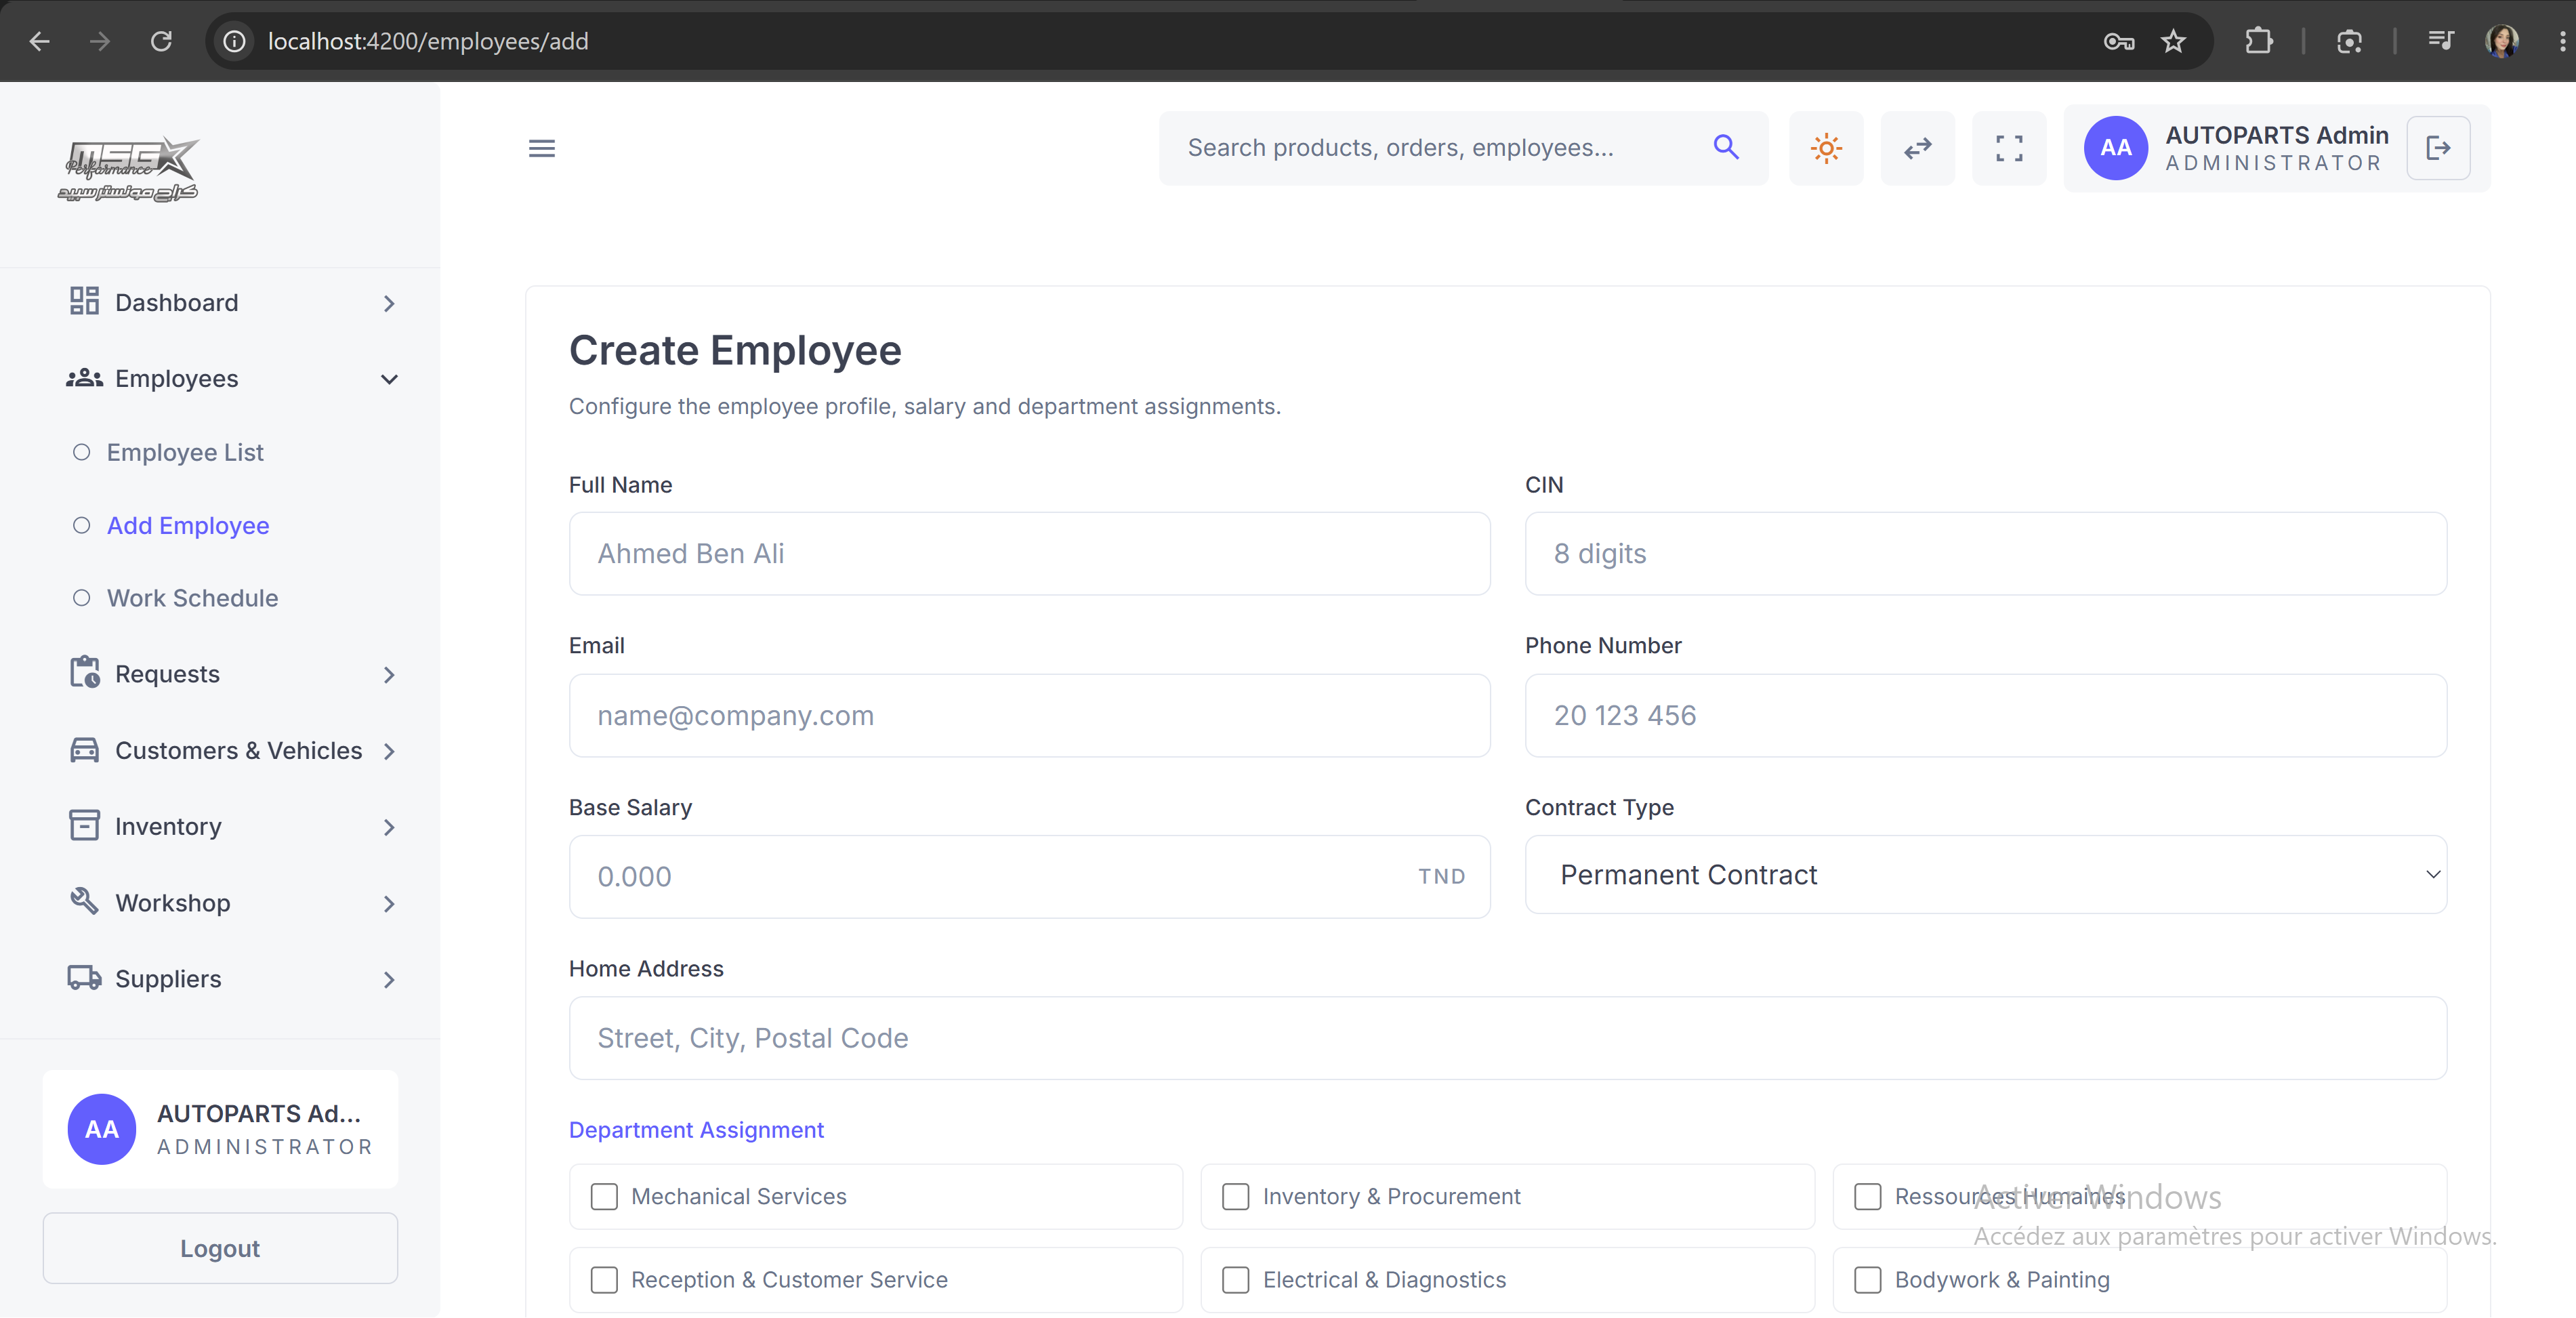
\includegraphics[width=\textwidth]{images/interfaces/AuthErp/CreationEmployee-ERP.png}
\caption{Interface de création d'un Employee}
\label{fig:createEmployee}
\end{figure}

Lors de la création, le système génère les informations de connexion initiales et les transmet automatiquement à l'employé par courrier électronique. Le compte est également initialisé avec l'état approprié afin de permettre sa première connexion.

À sa première connexion, l'employé utilise les identifiants reçus pour accéder à son espace de travail. Le système impose ensuite le changement du mot de passe initial afin de garantir la confidentialité des informations d'accès.

%---------------------------------------------------------





\section{Bilan du Sprint}

Ce premier sprint a permis de mettre en place les fondations de la gestion des
utilisateurs et de la sécurité de l'application AutoParts. Les principales
fonctionnalités d'authentification, d'inscription, de vérification des comptes,
de gestion des mots de passe et de création des employés ont été réalisées.
La mise en place de Spring Security et du JWT permet également de sécuriser
l'accès aux ressources et d'adapter les autorisations aux différents profils
et départements. Ce socle constitue ainsi une base fiable pour le développement
des fonctionnalités métiers des prochains sprints.